% EXTERNAL RESOURCES:
%   Resources should be stored in the "resources" folder, TeX or not,
%   including but not limited to:
%       - Images                    <- resources/images/...
%       - Figures                   <- resources/figures/...
%       - Tables                    <- resources/tables/...
%       - Listings (code snippets)  <- resources/code/...
%       - Bibliographies            <- resources/bibliography.bib
%       - Glossaries                <- resources/{acronyms.text}
%                                                 {glossary.tex}
%
%   Images **specifically** are stored relative to "resources/images"
%
%   Resource loading and imports are handled in the "include" folder,
%   you should define any imports in the "include/def_imports.tex" file.
%
% PART PREAMBLES:
%   When creating a part of more than 1 sub-part, e.g. not "title", it
%   is **highly** recommended you include a preamble TeX file of the
%   same name to handle any pre-processing, rather than in the first

%   subpart - this maintains the ethos of a modular library, and will
%   keep your project manageable!
%
% CREATING PARTS:
%   Use \include{} to include a new (set of) page(s) starting with a new
%   page right from the get-go automatically.
%
% CREATING SUB-PARTS:
%   Within pages, use \input{} to include sections etc., these do not
%   automatically add page-breaks, so any page-breaks still need to be
%   specified manually.
%
%   NOTE:
%       \input{} takes **absolute** paths, from the Overleaf root directory
%       onward to load from, "parts/title" is "parts/title" everywhere.
%-----------------------------------------------------------------------

\documentclass[12pt]{report}

% DO NOT USE THIS FILE UNLESS YOU KNOW WHAT YOU'RE DOING

\usepackage[export]{adjustbox}
%\usepackage[left=3.8cm,right=2.5cm,vmargin=3cm,footnotesep=0.5cm]{geometry}
\usepackage{geometry}
\geometry{
	paper=a4paper, % Paper size
	top=3cm, % Top margin
	bottom=2cm, % Bottom margin
	left=3.8cm, % Left margin
	right=2.5cm, % Right margin
	headheight=0.75cm, % Header height
	footskip=1.5cm, % Space from the bottom margin to the baseline of the footer
	headsep=0.75cm, % Space from the top margin to the baseline of the header
	%showframe, % Uncomment to show how the type block is set on the page
}
\usepackage{lipsum}
\usepackage{background}
\usepackage{listings}
\usepackage[automake, acronym, nonumberlist, nopostdot, toc, section=section]{glossaries}
\usepackage{xcolor}
\usepackage{hyperref}
\usepackage{enumitem}
\usepackage{amsmath}
\usepackage{amssymb}
\usepackage{multicol}
\usepackage{textcomp}
\usepackage{graphicx}
\usepackage{emoji}
\usepackage{babel}
\usepackage{titlesec}
\usepackage[backend=bibtex, style=ieee, sorting=ynt]{biblatex}
\usepackage{tikz}
\usetikzlibrary{calc}

% Removes the background for the specified page.
\newcommand\nobgpls{\backgroundsetup{contents={}}}

% Monospaced text within regular text for inline code
\newcommand{\code}{\texttt}

% Declares a figure with the given text underneath
%
% PARAMETERS:
%   #1  - figure label for referencing with \ref
%   #2  - figure content
%   #3  - figure caption
\newcommand{\namedfigure}[4]{
    \begin{figure}[#1]
        \label{#2}
        {\centering #3}
        \caption{#4}
    \end{figure}
}
\addbibresource{resources/bibliography.bib}
\graphicspath{{resources/images/}}
\glsenablehyper
\makeglossaries
% \newacronym[
%     description={Measure of legendary-osity.},
%     long={Legendary-ness Index Coefficient}
% ]

\newacronym{aic}{AIC}{Al-Azhar ICPC Community}
\newacronym{http}{HTTP}{HyperText Transfer Protocol}
\newacronym{ip}{IP}{Internet Protocol}
\newacronym{aes}{AES}{Advanced Encryption Standard}
\newacronym{cbc}{CBC}{Cipher block chaining}

% Consensus/Sybil-control
\newacronym{PoW}{PoW}{Proof of Work}
\newacronym{PoS}{PoS}{Proof of Stake}
\newacronym{PoA}{PoA}{Proof of Authority}

% Ethereum-related
\newacronym{nft}{nft}{Non-Fungible Token}
\newacronym{abi}{ABI}{Application Binary Interface}
\newacronym{evm}{EVM}{Ethereum Virtual Machine}
\newacronym{eth}{ETH}{Ether}
\newacronym{sc}{SC}{Smart Contract}
\newacronym{dapp}{DAPP}{Decentralized Application}

% Bitcoin-related

% Miscellaneous
\newacronym{dag}{DAG}{Directed Acyclic Graph}
\newacronym{asic}{ASIC}{Application-Specific Integrated Circuit}
\newacronym{tx}{TX}{Transaction}
\newacronym{p2p}{P2P}{Peer-to-Peer}

% IPFS-related
\newacronym{ipfs}{IPFS}{InterPlanetary File System}
\newacronym{acl}{ACL}{Access Control List}
\newacronym{cid}{CID}{Content Identifier}
\newacronym{dht}{DHT}{Distributed Hash Table}

% Blockchain Infurastructure
\newglossaryentry{blockchain} {
	name=blockchain,
	description={A blockchain is a distributed database that is shared among the nodes of a computer network. As a database, a blockchain stores information electronically in digital format.}
}

\newglossaryentry{block} {
	name=block,
	description={A block is a set of transactions that are recorded in a blockchain network.}
}

\newglossaryentry{chain} {
	name=chain,
	description={A chain is a sequence of blocks that are linked together by a hash of the previous block.}
}

\newglossaryentry{genesis} {
	name=genesis,
	description={The first block in a blockchain network.}
}

\newglossaryentry{consensus} {
	name=consensus,
	description={The process used by a group of peers, or nodes, on a blockchain network to agree on the validity of transactions submitted to the network. Dominant consensus mechanisms are Proof of Work (PoW) and Proof of Stake (PoS).}
}

\newglossaryentry{proof-of-work} {
	name=proof-of-work,
	description={Proof of work (PoW) is a form of cryptographic proof in which one party (the prover) proves to others (the verifiers) that a certain amount of a specific computational effort has been expended.}
}

\newglossaryentry{proof-of-stake} {
	name=proof-of-stake,
	description={Proof-of-stake (PoS) protocols are a class of consensus mechanisms for blockchains that work by selecting validators in proportion to their quantity of holdings in the associated cryptocurrency. This is done to avoid the computational cost of proof-of-work schemes.}
}

\newglossaryentry{mining} {
	name=mining,
	description={In a public blockchain, the process of verifying a transaction and writing it to the blockchain for which the successful miner is rewarded in the cryptocurrency of the blockchain.}
}

\newglossaryentry{nonce} {
	name=nonce,
	description={A nonce is an abbreviation for ``number only used once,'' which, in the context of cryptocurrency mining, is a number added to a hashed—or encrypted—block in a blockchain that, when rehashed, meets the difficulty level restrictions. The nonce is the number that blockchain miners are solving for. When the solution is found, the blockchain miners are offered cryptocurrency in exchange.}
}

\newglossaryentry{mainnet} {
	name=main net,
	description={The production version of a blockchain.}
}

\newglossaryentry{testnet} {
	name=test net,
	description={A staging blockchain environment for testing application before being put into production (or onto the mainnet).}
}

\newglossaryentry{node} {
	name=node,
	description={A computer which holds a copy of the blockchain ledger.}
}

\newglossaryentry{off-chain} {
	name=off-chain,
	description={Data stored external to the blockchain.}
}

\newglossaryentry{on-chain} {
	name=on-chain,
	description={Data stored within the blockchain.}
}


% Attacks
\newglossaryentry{51 attack} {
	name=51 attack,
	description={When more than 50\% of the miners in a blockchain launch an attack on the rest of the nodes/users to attempt to steal assets or double spend.}
}

% Cryptography and Security
\newglossaryentry{trustless} {
	name=trustless,
	description={The elimination of trust from a transaction.}
}

\newglossaryentry{immutable} {
	name=immutable,
	description={The property of being unchangeable. Once a transaction has been added to a block and written to a blockchain, it cannot be changed and therefore is immutable.}
}

\newglossaryentry{cryptography} {
	name=cryptography,
	description={The science of securing communication using individualized codes so only the participating parties can read the messages.}
}

\newglossaryentry{hash} {
	name=hash,
	description={A cryptographic hash function is a function that takes a message as input and produces a fixed-length output called a hash.}
}

\newglossaryentry{digital signature} {
	name=digital signature,
	description={A mathematical scheme for verifying digital messages or documents satisfy two requirements - they have authenticity and integrity.}
}

\newglossaryentry{wallet} {
	name=wallet,
	description={A digital file that holds coins and tokens held by the owner. The wallet also has a blockchain address to which transactions can be sent.}
}

\newglossaryentry{seed phrase} {
	name=seed phrase,
	description={A random sequence of words which can be used to restore a lost wallet.}
}

\newglossaryentry{public & private keys} {
	name=public key and private key,
	description={A public key is a unique string of characters derived from a private key which is used to encrypt a message or data. The private key is used to decrypt the message or data.}
}


% Bitcoin
\newglossaryentry{cryptocurrency} {
	name=cryptocurrency,
	description={Digital money which uses encryption and consensus algorithms to regulate the generation of coins/tokens and transfer of funds. Cryptocurrencies are generally decentralized, operating independently of central authorities.}
}

\newglossaryentry{bitcoin} {
	name=bitcoin,
	description={A cryptocurrency that uses a blockchain network to regulate the generation of coins/tokens and transfer of funds. Bitcoin is the most widely used cryptocurrency and is the most widely traded currency in the world.}
}

\newglossaryentry{satoshi nakamoto} {
	name=satoshi nakamoto,
	description={The name used by the person or entity who developed bitcoin, authored the bitcoin white paper, and created and deployed bitcoin's original reference implementation. As part of the implementation, Nakamoto also devised the first blockchain database.}
}


% Ethereum
\newglossaryentry{ethereum} {
	name=ethereum,
	description={A public blockchain that supports smart contracts.}
}

\newglossaryentry{smart contract} {
	name=smart contract,
	description={Self-executing computer code deployed on a blockchain to perform a function, often, but not always, the exchange of value between a buyer and a seller.}
}

\newglossaryentry{solidity} {
	name=solidity,
	description={Solidity is a programming language for smart contracts.}
}

\newglossaryentry{bytecode} {
	name=bytecode,
	description={Bytecode is the compiled code of a smart contract.}
}

\newglossaryentry{transaction} {
	name=transaction,
	description={A transaction is a set of instructions that are sent to a blockchain network to be processed by the network.}
}

\newglossaryentry{gas} {
	name=gas,
	description={A fee charged to write a transaction to a public blockchain. The gas is used to reward the miner which validates the transaction.}
}

\newglossaryentry{decentralized application} {
	name=dapp,
	description={Software which does not rely on a central system or database but can share information amongst its users via a decentralized database, such as a blockchain.}
}

% Miscellaneous
\newglossaryentry{open source} {
	name=open source,
	description={Software products that include permission to use, enhance, reuse or modify the source code, design documents, or content of the product.}
}

\newglossaryentry{peer-to-peer} {
	name=peer-to-peer,
	description={A direct connection between two participants in a system.}
}

\newglossaryentry{decentralized} {
	name=decentralization,
	description={A system with no single point where the decision is made. Every node makes a decision for its own behavior and the resulting system behavior is the aggregate response.}
}

\newglossaryentry{centralized} {
	name=centralized,
	description={A system or process for which there is a singular (i.e., central) source of authority, control and/or truth.}
}


% IPFS
\newglossaryentry{InterPlanetary file system} {
	name=ipfs,
	description={A peer-to-peer hypermedia protocol for the Internet. It is used to store and retrieve information in a decentralized way.}
}

\newglossaryentry{access-control list} {
	name=acl,
	description={In computer security, an access-control list (ACL) is a list of permissions associated with a system resource, also known as an object. An ACL specifies which users or system processes are granted access to objects, as well as what operations are allowed on given objects.}
}

\newglossaryentry{bitTorrent} {
	name=bitTorrent,
	description={BitTorrent is a communication protocol for peer-to-peer file sharing, which is used to distribute data and electronic files over the Internet.}
}

\newglossaryentry{content identifier} {
	name=cid,
	description={A Content Identifier (CID) is a self-describing content-addressed label used to point to the data stored in IPFS.}
}

\newglossaryentry{daemon} {
	name=daemon,
	description={A Daemon is a computer program that typically runs in the background. The IPFS daemon is how you take your node online to the IPFS network.}
}

\newglossaryentry{distributed hash table} {
	name=dht,
	description={A Distributed Hash Table (DHT) is a distributed key-value store where keys are cryptographic hashes. In IPFS, each peer is responsible for a subset of the IPFS DHT.}
}

\newglossaryentry{gateway} {
	name=gateway,
	description={An IPFS Gateway acts as a bridge between traditional web browsers and IPFS. Through the gateway, users can browse files and websites stored in IPFS as if they were stored on a traditional web server.}
}

\newglossaryentry{merkle tree} {
	name=merkle tree,
	description={A Merkle Tree is a specific type of hash tree used in cryptography and computer science, allowing efficient and secure verification of the contents of large data structures. Named after Ralph Merkle, who patented it in 1979.}
}

\geometry{
    a4paper,
    left=1in,
    right=1in,
    top=1in,
    bottom = 1in
}

\definecolor{codegreen}{rgb}{0,0.6,0}
\definecolor{codegray}{rgb}{0.5,0.5,0.5}
\definecolor{codepurple}{rgb}{0.58,0,0.82}
\definecolor{backcolour}{rgb}{0.95,0.95,0.92}

\lstdefinestyle{syntax-highlighted}{
    backgroundcolor=\color{backcolour},
    commentstyle=\color{codegreen},
    keywordstyle=\color{magenta},
    numberstyle=\tiny\color{codegray},
    stringstyle=\color{codepurple},
    basicstyle=\ttfamily\footnotesize,
    numberstyle=\ttfamily\Tiny,
    breakatwhitespace=false,
    breaklines=true,
    captionpos=b,
    keepspaces=true,
    numbers=none,
    numbersep=12pt,
    showspaces=false,
    showstringspaces=false,
    showtabs=false,
    tabsize=2
}

\lstset{style=syntax-highlighted}
\setacronymstyle{long-short-desc}


\begin{document}
	\nobgpls
\titleformat{\chapter}[display]
    {\normalfont\huge\bfseries}
    {\chaptertitlename\ \thechapter}
    {10pt}
    {\Huge}
\titlespacing*{\chapter}{0pt}{-32pt}{32pt}
	\begin{titlepage}
\centering

{
  \begin{center}
    
\includegraphics[scale=0.10]{cse.png}
  \end{center}
  \par
}
{\scshape\large Al-Azhar University\par}
{\scshape\Large Faculty of Engineering\par}
{\scshape\LARGE Computers \& Systems Engineering Department\par}
\vspace{2cm}\begin{titlepage}
\centering

{
  \begin{center}
    
\includegraphics[scale=0.10]{cse.png}
  \end{center}
  \par
}
{\scshape\large Al-Azhar University\par}
{\scshape\Large Faculty of Engineering\par}
{\scshape\LARGE Computers \& Systems Engineering Department\par}
\vspace{2cm}\begin{titlepage}
\centering

\input{parts/title/header}
\vspace{2cm}\input{parts/title/title}
\vspace{3cm}\input{parts/title/award}
\vspace{2cm}\input{parts/title/name}
\vspace{2cm}\input{parts/title/supervisors}
\vspace{1cm}\input{parts/title/date}

\end{titlepage}
\vspace{3cm}{
  \large
  \sffamily
  % \textsc{Bachelor Thesis}
  \textsc{A Project Submitted in Partial Fulfillment of the Requirements for the Degree of Bachelor of Science in Systems and Computers Engineering}
  \par
}
\vspace{2cm}{
  \centering
  \Large
  \textsl{Submitted by:} \\
  \bfseries
  {
    \begin{tabular}{lr}
      Abd El-Twab M. Fakhry & \textsl{504055} \\
      Hossam A. Eissa & \textsl{504042}
    \end{tabular}
  }
  \par
}
\vspace{2cm}{
  \centering
  \Large
  \textsl{Supervised by:}\\
  \textbf{Dr. Abdurrahman Nasr}
  \par
}

\vspace{1cm}{
  \textsc
  \today
  \par
}

\end{titlepage}
\vspace{3cm}{
  \large
  \sffamily
  % \textsc{Bachelor Thesis}
  \textsc{A Project Submitted in Partial Fulfillment of the Requirements for the Degree of Bachelor of Science in Systems and Computers Engineering}
  \par
}
\vspace{2cm}{
  \centering
  \Large
  \textsl{Submitted by:} \\
  \bfseries
  {
    \begin{tabular}{lr}
      Abd El-Twab M. Fakhry & \textsl{504055} \\
      Hossam A. Eissa & \textsl{504042}
    \end{tabular}
  }
  \par
}
\vspace{2cm}{
  \centering
  \Large
  \textsl{Supervised by:}\\
  \textbf{Dr. Abdurrahman Nasr}
  \par
}

\vspace{1cm}{
  \textsc
  \today
  \par
}

\end{titlepage}
  \afterpage{\blankpage}
	\pagenumbering{roman}
	%%% Local Variables:
%%% mode: latex
%%% TeX-master: t
%%% End:

\chapter*{Letter of Approval}
\addcontentsline{toc}{chapter}{Letter of Approval}

The undersigned certify that they have read, and recommended to the Faculty of Engineering for acceptance, a project entitled ``Devault: A Blockchain-based, self-hosted, and end-to-end encrypted cloud storage'' submitted by Abd El-Twab M. Fakhry and Hossam A. Eissa in partial fulfillment of the requirements for the degree of Bachelor of Science in Systems and Computers Engineering.\vspace{2cm}


\begin{center}
  \par\noindent\rule{0.50\textwidth}{0.4pt}\par
  \footnotesize
  Examiner Committee President:\par\vspace{4pt}
  \normalsize
  Dr. Ali ElSamary\par\vspace{4pt}
  \footnotesize
  \scshape
  Systems \& Computers Engineering Department\par
\end{center}\vspace{16pt}
\begin{multicols}{2}
  \begin{center}
    \par\noindent\rule{0.40\textwidth}{0.4pt}\par
    \footnotesize
    Project Supervisor:\par\vspace{4pt}
    \normalsize
    Dr. Abdurrahman Nasr\par\vspace{4pt}
    \footnotesize
    \scshape
    Systems \& Computers Engineering Department\par
  \end{center}
  \begin{center}
    \par\noindent\rule{0.40\textwidth}{0.4pt}\par
    \footnotesize
    Examiner Member:\par\vspace{4pt}
    \normalsize
    Dr. Muhammad Atef\par\vspace{4pt}
    \footnotesize
    \scshape
    Systems \& Computers Engineering Department\par
  \end{center}
\end{multicols}\vspace{2cm}
{
  \Large
  \textsl{Date of Approval:}
}
  \chapter*{Statement of Originality}
\addcontentsline{toc}{chapter}{Statement of Originality}

This statement is to certify that to the best of our knowledge, the content of this thesis is our work. This thesis has not been submitted for any degree or other purposes. \\[4pt]
\noindent
We certify that the intellectual content of this thesis is the product of our work and that all the assistance received in preparing this thesis and sources has been acknowledged. \\[8pt]

\begin{flushright}
  \itshape
  \par\noindent\rule{0.30\textwidth}{0.4pt}\par
  Abd El-Twab M. Fakhry\par
  Hossam A. Eissa \\[8pt]

  \footnotesize
  \normalshape
  \today
\end{flushright}

  {
  \centering
  \bfseries
  To the person who helped...
}
  \chapter*{Acknowledgements}
\addcontentsline{toc}{chapter}{Acknowledgements}

\noindent
In successfully completing this project, many people have helped me. I would like to thank all those who are related to this project. \\[4pt]

Primarily, thanks to ALLAH (s.w.t), the Greatest, the Most Merciful, and the Most Gracious,
Whose countless blessings bestowed upon me were kind, talented, and wise teachers, who
provided me with sufficient opportunities and enlighten me towards this project. \\[4pt]

I would like to express my deepest and most sincere gratitude to my family for everything they have done for me and all the love they gave to me. My mother, father, sisters, and brother. No words can express my love for them. \\[4pt]

I would like to extend my deepest thanks to my supervisor, Dr. Abdurrahman Nasr for
giving me the opportunity of undertaking this research work under his determined
direction. His support, dedication, encouragement, excellent supervision, and guidance
are what made this thesis possible. \\[4pt]

Last but not least, I would like to thank my friends and colleagues, especially \acrfull{aic} team members, who have helped me with their valuable suggestions and guidance and have been very helpful in various stages of project completion. \\[16pt]

\noindent
Thank You.
  \chapter*{Abstract}
\addcontentsline{toc}{chapter}{Abstract}

We propose a \acrfull{dapp} that uses the \Gls{ethereum} \gls{smart contract}s for data access control and uses the \acrfull{ipfs} as a distributed system for storing and accessing data. Moreover, the files get encrypted on the client side using \acrshort{aes}-256-\acrshort{cbc} symmetric encryption and split into smaller chunks, distributed across multiple computers, and assigned a hash to allow users to locate them. It’s then served to the user via a peer-to-peer connection, similar to BitTorrent technology.

Our proposed solution overcomes the problem of the \gls{centralized} web, data censorship, data hacking, and data loss.

\vspace{1cm}
\noindent
\textsc{Keywords}: \textsl{ Blockchain; Cryptology; Peer-to-Peer Network; Decentralised Applications; Cloud Computing}

	\tableofcontents

  % EXTERNAL RESOURCES:
%   Resources should be stored in the "resources" folder, TeX or not,
%   including but not limited to:
%       - Images                    <- resources/images/...
%       - Figures                   <- resources/figures/...
%       - Tables                    <- resources/tables/...
%       - Listings (code snippets)  <- resources/code/...
%       - Bibliographies            <- resources/bibliography.bib
%       - Glossaries                <- resources/{acronyms.text}
%                                                 {glossary.tex}
%
%   Images **specifically** are stored relative to "resources/images"
%
%   Resource loading and imports are handled in the "include" folder,
%   you should define any imports in the "include/def_imports.tex" file.
%
% PART PREAMBLES:
%   When creating a part of more than 1 sub-part, e.g. not "title", it
%   is **highly** recommended you include a preamble TeX file of the
%   same name to handle any pre-processing, rather than in the first

%   subpart - this maintains the ethos of a modular library, and will
%   keep your project manageable!
%
% CREATING PARTS:
%   Use \include{} to include a new (set of) page(s) starting with a new
%   page right from the get-go automatically.
%
% CREATING SUB-PARTS:
%   Within pages, use \input{} to include sections etc., these do not
%   automatically add page-breaks, so any page-breaks still need to be
%   specified manually.
%
%   NOTE:
%       \input{} takes **absolute** paths, from the Overleaf root directory
%       onward to load from, "parts/title" is "parts/title" everywhere.
%-----------------------------------------------------------------------

\documentclass[12pt]{report}

% DO NOT USE THIS FILE UNLESS YOU KNOW WHAT YOU'RE DOING

\usepackage[export]{adjustbox}
%\usepackage[left=3.8cm,right=2.5cm,vmargin=3cm,footnotesep=0.5cm]{geometry}
\usepackage{geometry}
\geometry{
	paper=a4paper, % Paper size
	top=3cm, % Top margin
	bottom=2cm, % Bottom margin
	left=3.8cm, % Left margin
	right=2.5cm, % Right margin
	headheight=0.75cm, % Header height
	footskip=1.5cm, % Space from the bottom margin to the baseline of the footer
	headsep=0.75cm, % Space from the top margin to the baseline of the header
	%showframe, % Uncomment to show how the type block is set on the page
}
\usepackage{lipsum}
\usepackage{background}
\usepackage{listings}
\usepackage[automake, acronym, nonumberlist, nopostdot, toc, section=section]{glossaries}
\usepackage{xcolor}
\usepackage{hyperref}
\usepackage{enumitem}
\usepackage{amsmath}
\usepackage{amssymb}
\usepackage{multicol}
\usepackage{textcomp}
\usepackage{graphicx}
\usepackage{emoji}
\usepackage{babel}
\usepackage{titlesec}
\usepackage[backend=bibtex, style=ieee, sorting=ynt]{biblatex}
\usepackage{tikz}
\usetikzlibrary{calc}

% Removes the background for the specified page.
\newcommand\nobgpls{\backgroundsetup{contents={}}}

% Monospaced text within regular text for inline code
\newcommand{\code}{\texttt}

% Declares a figure with the given text underneath
%
% PARAMETERS:
%   #1  - figure label for referencing with \ref
%   #2  - figure content
%   #3  - figure caption
\newcommand{\namedfigure}[4]{
    \begin{figure}[#1]
        \label{#2}
        {\centering #3}
        \caption{#4}
    \end{figure}
}
\addbibresource{resources/bibliography.bib}
\graphicspath{{resources/images/}}
\glsenablehyper
\makeglossaries
% \newacronym[
%     description={Measure of legendary-osity.},
%     long={Legendary-ness Index Coefficient}
% ]

\newacronym{aic}{AIC}{Al-Azhar ICPC Community}
\newacronym{http}{HTTP}{HyperText Transfer Protocol}
\newacronym{ip}{IP}{Internet Protocol}
\newacronym{aes}{AES}{Advanced Encryption Standard}
\newacronym{cbc}{CBC}{Cipher block chaining}

% Consensus/Sybil-control
\newacronym{PoW}{PoW}{Proof of Work}
\newacronym{PoS}{PoS}{Proof of Stake}
\newacronym{PoA}{PoA}{Proof of Authority}

% Ethereum-related
\newacronym{nft}{nft}{Non-Fungible Token}
\newacronym{abi}{ABI}{Application Binary Interface}
\newacronym{evm}{EVM}{Ethereum Virtual Machine}
\newacronym{eth}{ETH}{Ether}
\newacronym{sc}{SC}{Smart Contract}
\newacronym{dapp}{DAPP}{Decentralized Application}

% Bitcoin-related

% Miscellaneous
\newacronym{dag}{DAG}{Directed Acyclic Graph}
\newacronym{asic}{ASIC}{Application-Specific Integrated Circuit}
\newacronym{tx}{TX}{Transaction}
\newacronym{p2p}{P2P}{Peer-to-Peer}

% IPFS-related
\newacronym{ipfs}{IPFS}{InterPlanetary File System}
\newacronym{acl}{ACL}{Access Control List}
\newacronym{cid}{CID}{Content Identifier}
\newacronym{dht}{DHT}{Distributed Hash Table}

% Blockchain Infurastructure
\newglossaryentry{blockchain} {
	name=blockchain,
	description={A blockchain is a distributed database that is shared among the nodes of a computer network. As a database, a blockchain stores information electronically in digital format.}
}

\newglossaryentry{block} {
	name=block,
	description={A block is a set of transactions that are recorded in a blockchain network.}
}

\newglossaryentry{chain} {
	name=chain,
	description={A chain is a sequence of blocks that are linked together by a hash of the previous block.}
}

\newglossaryentry{genesis} {
	name=genesis,
	description={The first block in a blockchain network.}
}

\newglossaryentry{consensus} {
	name=consensus,
	description={The process used by a group of peers, or nodes, on a blockchain network to agree on the validity of transactions submitted to the network. Dominant consensus mechanisms are Proof of Work (PoW) and Proof of Stake (PoS).}
}

\newglossaryentry{proof-of-work} {
	name=proof-of-work,
	description={Proof of work (PoW) is a form of cryptographic proof in which one party (the prover) proves to others (the verifiers) that a certain amount of a specific computational effort has been expended.}
}

\newglossaryentry{proof-of-stake} {
	name=proof-of-stake,
	description={Proof-of-stake (PoS) protocols are a class of consensus mechanisms for blockchains that work by selecting validators in proportion to their quantity of holdings in the associated cryptocurrency. This is done to avoid the computational cost of proof-of-work schemes.}
}

\newglossaryentry{mining} {
	name=mining,
	description={In a public blockchain, the process of verifying a transaction and writing it to the blockchain for which the successful miner is rewarded in the cryptocurrency of the blockchain.}
}

\newglossaryentry{nonce} {
	name=nonce,
	description={A nonce is an abbreviation for ``number only used once,'' which, in the context of cryptocurrency mining, is a number added to a hashed—or encrypted—block in a blockchain that, when rehashed, meets the difficulty level restrictions. The nonce is the number that blockchain miners are solving for. When the solution is found, the blockchain miners are offered cryptocurrency in exchange.}
}

\newglossaryentry{mainnet} {
	name=main net,
	description={The production version of a blockchain.}
}

\newglossaryentry{testnet} {
	name=test net,
	description={A staging blockchain environment for testing application before being put into production (or onto the mainnet).}
}

\newglossaryentry{node} {
	name=node,
	description={A computer which holds a copy of the blockchain ledger.}
}

\newglossaryentry{off-chain} {
	name=off-chain,
	description={Data stored external to the blockchain.}
}

\newglossaryentry{on-chain} {
	name=on-chain,
	description={Data stored within the blockchain.}
}


% Attacks
\newglossaryentry{51 attack} {
	name=51 attack,
	description={When more than 50\% of the miners in a blockchain launch an attack on the rest of the nodes/users to attempt to steal assets or double spend.}
}

% Cryptography and Security
\newglossaryentry{trustless} {
	name=trustless,
	description={The elimination of trust from a transaction.}
}

\newglossaryentry{immutable} {
	name=immutable,
	description={The property of being unchangeable. Once a transaction has been added to a block and written to a blockchain, it cannot be changed and therefore is immutable.}
}

\newglossaryentry{cryptography} {
	name=cryptography,
	description={The science of securing communication using individualized codes so only the participating parties can read the messages.}
}

\newglossaryentry{hash} {
	name=hash,
	description={A cryptographic hash function is a function that takes a message as input and produces a fixed-length output called a hash.}
}

\newglossaryentry{digital signature} {
	name=digital signature,
	description={A mathematical scheme for verifying digital messages or documents satisfy two requirements - they have authenticity and integrity.}
}

\newglossaryentry{wallet} {
	name=wallet,
	description={A digital file that holds coins and tokens held by the owner. The wallet also has a blockchain address to which transactions can be sent.}
}

\newglossaryentry{seed phrase} {
	name=seed phrase,
	description={A random sequence of words which can be used to restore a lost wallet.}
}

\newglossaryentry{public & private keys} {
	name=public key and private key,
	description={A public key is a unique string of characters derived from a private key which is used to encrypt a message or data. The private key is used to decrypt the message or data.}
}


% Bitcoin
\newglossaryentry{cryptocurrency} {
	name=cryptocurrency,
	description={Digital money which uses encryption and consensus algorithms to regulate the generation of coins/tokens and transfer of funds. Cryptocurrencies are generally decentralized, operating independently of central authorities.}
}

\newglossaryentry{bitcoin} {
	name=bitcoin,
	description={A cryptocurrency that uses a blockchain network to regulate the generation of coins/tokens and transfer of funds. Bitcoin is the most widely used cryptocurrency and is the most widely traded currency in the world.}
}

\newglossaryentry{satoshi nakamoto} {
	name=satoshi nakamoto,
	description={The name used by the person or entity who developed bitcoin, authored the bitcoin white paper, and created and deployed bitcoin's original reference implementation. As part of the implementation, Nakamoto also devised the first blockchain database.}
}


% Ethereum
\newglossaryentry{ethereum} {
	name=ethereum,
	description={A public blockchain that supports smart contracts.}
}

\newglossaryentry{smart contract} {
	name=smart contract,
	description={Self-executing computer code deployed on a blockchain to perform a function, often, but not always, the exchange of value between a buyer and a seller.}
}

\newglossaryentry{solidity} {
	name=solidity,
	description={Solidity is a programming language for smart contracts.}
}

\newglossaryentry{bytecode} {
	name=bytecode,
	description={Bytecode is the compiled code of a smart contract.}
}

\newglossaryentry{transaction} {
	name=transaction,
	description={A transaction is a set of instructions that are sent to a blockchain network to be processed by the network.}
}

\newglossaryentry{gas} {
	name=gas,
	description={A fee charged to write a transaction to a public blockchain. The gas is used to reward the miner which validates the transaction.}
}

\newglossaryentry{decentralized application} {
	name=dapp,
	description={Software which does not rely on a central system or database but can share information amongst its users via a decentralized database, such as a blockchain.}
}

% Miscellaneous
\newglossaryentry{open source} {
	name=open source,
	description={Software products that include permission to use, enhance, reuse or modify the source code, design documents, or content of the product.}
}

\newglossaryentry{peer-to-peer} {
	name=peer-to-peer,
	description={A direct connection between two participants in a system.}
}

\newglossaryentry{decentralized} {
	name=decentralization,
	description={A system with no single point where the decision is made. Every node makes a decision for its own behavior and the resulting system behavior is the aggregate response.}
}

\newglossaryentry{centralized} {
	name=centralized,
	description={A system or process for which there is a singular (i.e., central) source of authority, control and/or truth.}
}


% IPFS
\newglossaryentry{InterPlanetary file system} {
	name=ipfs,
	description={A peer-to-peer hypermedia protocol for the Internet. It is used to store and retrieve information in a decentralized way.}
}

\newglossaryentry{access-control list} {
	name=acl,
	description={In computer security, an access-control list (ACL) is a list of permissions associated with a system resource, also known as an object. An ACL specifies which users or system processes are granted access to objects, as well as what operations are allowed on given objects.}
}

\newglossaryentry{bitTorrent} {
	name=bitTorrent,
	description={BitTorrent is a communication protocol for peer-to-peer file sharing, which is used to distribute data and electronic files over the Internet.}
}

\newglossaryentry{content identifier} {
	name=cid,
	description={A Content Identifier (CID) is a self-describing content-addressed label used to point to the data stored in IPFS.}
}

\newglossaryentry{daemon} {
	name=daemon,
	description={A Daemon is a computer program that typically runs in the background. The IPFS daemon is how you take your node online to the IPFS network.}
}

\newglossaryentry{distributed hash table} {
	name=dht,
	description={A Distributed Hash Table (DHT) is a distributed key-value store where keys are cryptographic hashes. In IPFS, each peer is responsible for a subset of the IPFS DHT.}
}

\newglossaryentry{gateway} {
	name=gateway,
	description={An IPFS Gateway acts as a bridge between traditional web browsers and IPFS. Through the gateway, users can browse files and websites stored in IPFS as if they were stored on a traditional web server.}
}

\newglossaryentry{merkle tree} {
	name=merkle tree,
	description={A Merkle Tree is a specific type of hash tree used in cryptography and computer science, allowing efficient and secure verification of the contents of large data structures. Named after Ralph Merkle, who patented it in 1979.}
}

\geometry{
    a4paper,
    left=1in,
    right=1in,
    top=1in,
    bottom = 1in
}

\definecolor{codegreen}{rgb}{0,0.6,0}
\definecolor{codegray}{rgb}{0.5,0.5,0.5}
\definecolor{codepurple}{rgb}{0.58,0,0.82}
\definecolor{backcolour}{rgb}{0.95,0.95,0.92}

\lstdefinestyle{syntax-highlighted}{
    backgroundcolor=\color{backcolour},
    commentstyle=\color{codegreen},
    keywordstyle=\color{magenta},
    numberstyle=\tiny\color{codegray},
    stringstyle=\color{codepurple},
    basicstyle=\ttfamily\footnotesize,
    numberstyle=\ttfamily\Tiny,
    breakatwhitespace=false,
    breaklines=true,
    captionpos=b,
    keepspaces=true,
    numbers=none,
    numbersep=12pt,
    showspaces=false,
    showstringspaces=false,
    showtabs=false,
    tabsize=2
}

\lstset{style=syntax-highlighted}
\setacronymstyle{long-short-desc}


\begin{document}
	\nobgpls
\titleformat{\chapter}[display]
    {\normalfont\huge\bfseries}
    {\chaptertitlename\ \thechapter}
    {10pt}
    {\Huge}
\titlespacing*{\chapter}{0pt}{-32pt}{32pt}
	\begin{titlepage}
\centering

{
  \begin{center}
    
\includegraphics[scale=0.10]{cse.png}
  \end{center}
  \par
}
{\scshape\large Al-Azhar University\par}
{\scshape\Large Faculty of Engineering\par}
{\scshape\LARGE Computers \& Systems Engineering Department\par}
\vspace{2cm}\begin{titlepage}
\centering

\input{parts/title/header}
\vspace{2cm}\input{parts/title/title}
\vspace{3cm}\input{parts/title/award}
\vspace{2cm}\input{parts/title/name}
\vspace{2cm}\input{parts/title/supervisors}
\vspace{1cm}\input{parts/title/date}

\end{titlepage}
\vspace{3cm}{
  \large
  \sffamily
  % \textsc{Bachelor Thesis}
  \textsc{A Project Submitted in Partial Fulfillment of the Requirements for the Degree of Bachelor of Science in Systems and Computers Engineering}
  \par
}
\vspace{2cm}{
  \centering
  \Large
  \textsl{Submitted by:} \\
  \bfseries
  {
    \begin{tabular}{lr}
      Abd El-Twab M. Fakhry & \textsl{504055} \\
      Hossam A. Eissa & \textsl{504042}
    \end{tabular}
  }
  \par
}
\vspace{2cm}{
  \centering
  \Large
  \textsl{Supervised by:}\\
  \textbf{Dr. Abdurrahman Nasr}
  \par
}

\vspace{1cm}{
  \textsc
  \today
  \par
}

\end{titlepage}
  \afterpage{\blankpage}
	\pagenumbering{roman}
	%%% Local Variables:
%%% mode: latex
%%% TeX-master: t
%%% End:

\chapter*{Letter of Approval}
\addcontentsline{toc}{chapter}{Letter of Approval}

The undersigned certify that they have read, and recommended to the Faculty of Engineering for acceptance, a project entitled ``Devault: A Blockchain-based, self-hosted, and end-to-end encrypted cloud storage'' submitted by Abd El-Twab M. Fakhry and Hossam A. Eissa in partial fulfillment of the requirements for the degree of Bachelor of Science in Systems and Computers Engineering.\vspace{2cm}


\begin{center}
  \par\noindent\rule{0.50\textwidth}{0.4pt}\par
  \footnotesize
  Examiner Committee President:\par\vspace{4pt}
  \normalsize
  Dr. Ali ElSamary\par\vspace{4pt}
  \footnotesize
  \scshape
  Systems \& Computers Engineering Department\par
\end{center}\vspace{16pt}
\begin{multicols}{2}
  \begin{center}
    \par\noindent\rule{0.40\textwidth}{0.4pt}\par
    \footnotesize
    Project Supervisor:\par\vspace{4pt}
    \normalsize
    Dr. Abdurrahman Nasr\par\vspace{4pt}
    \footnotesize
    \scshape
    Systems \& Computers Engineering Department\par
  \end{center}
  \begin{center}
    \par\noindent\rule{0.40\textwidth}{0.4pt}\par
    \footnotesize
    Examiner Member:\par\vspace{4pt}
    \normalsize
    Dr. Muhammad Atef\par\vspace{4pt}
    \footnotesize
    \scshape
    Systems \& Computers Engineering Department\par
  \end{center}
\end{multicols}\vspace{2cm}
{
  \Large
  \textsl{Date of Approval:}
}
  \chapter*{Statement of Originality}
\addcontentsline{toc}{chapter}{Statement of Originality}

This statement is to certify that to the best of our knowledge, the content of this thesis is our work. This thesis has not been submitted for any degree or other purposes. \\[4pt]
\noindent
We certify that the intellectual content of this thesis is the product of our work and that all the assistance received in preparing this thesis and sources has been acknowledged. \\[8pt]

\begin{flushright}
  \itshape
  \par\noindent\rule{0.30\textwidth}{0.4pt}\par
  Abd El-Twab M. Fakhry\par
  Hossam A. Eissa \\[8pt]

  \footnotesize
  \normalshape
  \today
\end{flushright}

  {
  \centering
  \bfseries
  To the person who helped...
}
  \chapter*{Acknowledgements}
\addcontentsline{toc}{chapter}{Acknowledgements}

\noindent
In successfully completing this project, many people have helped me. I would like to thank all those who are related to this project. \\[4pt]

Primarily, thanks to ALLAH (s.w.t), the Greatest, the Most Merciful, and the Most Gracious,
Whose countless blessings bestowed upon me were kind, talented, and wise teachers, who
provided me with sufficient opportunities and enlighten me towards this project. \\[4pt]

I would like to express my deepest and most sincere gratitude to my family for everything they have done for me and all the love they gave to me. My mother, father, sisters, and brother. No words can express my love for them. \\[4pt]

I would like to extend my deepest thanks to my supervisor, Dr. Abdurrahman Nasr for
giving me the opportunity of undertaking this research work under his determined
direction. His support, dedication, encouragement, excellent supervision, and guidance
are what made this thesis possible. \\[4pt]

Last but not least, I would like to thank my friends and colleagues, especially \acrfull{aic} team members, who have helped me with their valuable suggestions and guidance and have been very helpful in various stages of project completion. \\[16pt]

\noindent
Thank You.
  \chapter*{Abstract}
\addcontentsline{toc}{chapter}{Abstract}

We propose a \acrfull{dapp} that uses the \Gls{ethereum} \gls{smart contract}s for data access control and uses the \acrfull{ipfs} as a distributed system for storing and accessing data. Moreover, the files get encrypted on the client side using \acrshort{aes}-256-\acrshort{cbc} symmetric encryption and split into smaller chunks, distributed across multiple computers, and assigned a hash to allow users to locate them. It’s then served to the user via a peer-to-peer connection, similar to BitTorrent technology.

Our proposed solution overcomes the problem of the \gls{centralized} web, data censorship, data hacking, and data loss.

\vspace{1cm}
\noindent
\textsc{Keywords}: \textsl{ Blockchain; Cryptology; Peer-to-Peer Network; Decentralised Applications; Cloud Computing}

	\tableofcontents

  % EXTERNAL RESOURCES:
%   Resources should be stored in the "resources" folder, TeX or not,
%   including but not limited to:
%       - Images                    <- resources/images/...
%       - Figures                   <- resources/figures/...
%       - Tables                    <- resources/tables/...
%       - Listings (code snippets)  <- resources/code/...
%       - Bibliographies            <- resources/bibliography.bib
%       - Glossaries                <- resources/{acronyms.text}
%                                                 {glossary.tex}
%
%   Images **specifically** are stored relative to "resources/images"
%
%   Resource loading and imports are handled in the "include" folder,
%   you should define any imports in the "include/def_imports.tex" file.
%
% PART PREAMBLES:
%   When creating a part of more than 1 sub-part, e.g. not "title", it
%   is **highly** recommended you include a preamble TeX file of the
%   same name to handle any pre-processing, rather than in the first

%   subpart - this maintains the ethos of a modular library, and will
%   keep your project manageable!
%
% CREATING PARTS:
%   Use \include{} to include a new (set of) page(s) starting with a new
%   page right from the get-go automatically.
%
% CREATING SUB-PARTS:
%   Within pages, use \input{} to include sections etc., these do not
%   automatically add page-breaks, so any page-breaks still need to be
%   specified manually.
%
%   NOTE:
%       \input{} takes **absolute** paths, from the Overleaf root directory
%       onward to load from, "parts/title" is "parts/title" everywhere.
%-----------------------------------------------------------------------

\documentclass[12pt]{report}

% DO NOT USE THIS FILE UNLESS YOU KNOW WHAT YOU'RE DOING

\usepackage[export]{adjustbox}
%\usepackage[left=3.8cm,right=2.5cm,vmargin=3cm,footnotesep=0.5cm]{geometry}
\usepackage{geometry}
\geometry{
	paper=a4paper, % Paper size
	top=3cm, % Top margin
	bottom=2cm, % Bottom margin
	left=3.8cm, % Left margin
	right=2.5cm, % Right margin
	headheight=0.75cm, % Header height
	footskip=1.5cm, % Space from the bottom margin to the baseline of the footer
	headsep=0.75cm, % Space from the top margin to the baseline of the header
	%showframe, % Uncomment to show how the type block is set on the page
}
\usepackage{lipsum}
\usepackage{background}
\usepackage{listings}
\usepackage[automake, acronym, nonumberlist, nopostdot, toc, section=section]{glossaries}
\usepackage{xcolor}
\usepackage{hyperref}
\usepackage{enumitem}
\usepackage{amsmath}
\usepackage{amssymb}
\usepackage{multicol}
\usepackage{textcomp}
\usepackage{graphicx}
\usepackage{emoji}
\usepackage{babel}
\usepackage{titlesec}
\usepackage[backend=bibtex, style=ieee, sorting=ynt]{biblatex}
\usepackage{tikz}
\usetikzlibrary{calc}

% Removes the background for the specified page.
\newcommand\nobgpls{\backgroundsetup{contents={}}}

% Monospaced text within regular text for inline code
\newcommand{\code}{\texttt}

% Declares a figure with the given text underneath
%
% PARAMETERS:
%   #1  - figure label for referencing with \ref
%   #2  - figure content
%   #3  - figure caption
\newcommand{\namedfigure}[4]{
    \begin{figure}[#1]
        \label{#2}
        {\centering #3}
        \caption{#4}
    \end{figure}
}
\addbibresource{resources/bibliography.bib}
\graphicspath{{resources/images/}}
\glsenablehyper
\makeglossaries
\input{resources/acronyms}
\input{resources/glossary}
\geometry{
    a4paper,
    left=1in,
    right=1in,
    top=1in,
    bottom = 1in
}

\definecolor{codegreen}{rgb}{0,0.6,0}
\definecolor{codegray}{rgb}{0.5,0.5,0.5}
\definecolor{codepurple}{rgb}{0.58,0,0.82}
\definecolor{backcolour}{rgb}{0.95,0.95,0.92}

\lstdefinestyle{syntax-highlighted}{
    backgroundcolor=\color{backcolour},
    commentstyle=\color{codegreen},
    keywordstyle=\color{magenta},
    numberstyle=\tiny\color{codegray},
    stringstyle=\color{codepurple},
    basicstyle=\ttfamily\footnotesize,
    numberstyle=\ttfamily\Tiny,
    breakatwhitespace=false,
    breaklines=true,
    captionpos=b,
    keepspaces=true,
    numbers=none,
    numbersep=12pt,
    showspaces=false,
    showstringspaces=false,
    showtabs=false,
    tabsize=2
}

\lstset{style=syntax-highlighted}
\setacronymstyle{long-short-desc}


\begin{document}
	\nobgpls
\titleformat{\chapter}[display]
    {\normalfont\huge\bfseries}
    {\chaptertitlename\ \thechapter}
    {10pt}
    {\Huge}
\titlespacing*{\chapter}{0pt}{-32pt}{32pt}
	\begin{titlepage}
\centering

\input{parts/title/header}
\vspace{2cm}\input{parts/title/title}
\vspace{3cm}\input{parts/title/award}
\vspace{2cm}\input{parts/title/name}
\vspace{2cm}\input{parts/title/supervisors}
\vspace{1cm}\input{parts/title/date}

\end{titlepage}
  \afterpage{\blankpage}
	\pagenumbering{roman}
	%%% Local Variables:
%%% mode: latex
%%% TeX-master: t
%%% End:

\chapter*{Letter of Approval}
\addcontentsline{toc}{chapter}{Letter of Approval}

The undersigned certify that they have read, and recommended to the Faculty of Engineering for acceptance, a project entitled ``Devault: A Blockchain-based, self-hosted, and end-to-end encrypted cloud storage'' submitted by Abd El-Twab M. Fakhry and Hossam A. Eissa in partial fulfillment of the requirements for the degree of Bachelor of Science in Systems and Computers Engineering.\vspace{2cm}


\begin{center}
  \par\noindent\rule{0.50\textwidth}{0.4pt}\par
  \footnotesize
  Examiner Committee President:\par\vspace{4pt}
  \normalsize
  Dr. Ali ElSamary\par\vspace{4pt}
  \footnotesize
  \scshape
  Systems \& Computers Engineering Department\par
\end{center}\vspace{16pt}
\begin{multicols}{2}
  \begin{center}
    \par\noindent\rule{0.40\textwidth}{0.4pt}\par
    \footnotesize
    Project Supervisor:\par\vspace{4pt}
    \normalsize
    Dr. Abdurrahman Nasr\par\vspace{4pt}
    \footnotesize
    \scshape
    Systems \& Computers Engineering Department\par
  \end{center}
  \begin{center}
    \par\noindent\rule{0.40\textwidth}{0.4pt}\par
    \footnotesize
    Examiner Member:\par\vspace{4pt}
    \normalsize
    Dr. Muhammad Atef\par\vspace{4pt}
    \footnotesize
    \scshape
    Systems \& Computers Engineering Department\par
  \end{center}
\end{multicols}\vspace{2cm}
{
  \Large
  \textsl{Date of Approval:}
}
  \chapter*{Statement of Originality}
\addcontentsline{toc}{chapter}{Statement of Originality}

This statement is to certify that to the best of our knowledge, the content of this thesis is our work. This thesis has not been submitted for any degree or other purposes. \\[4pt]
\noindent
We certify that the intellectual content of this thesis is the product of our work and that all the assistance received in preparing this thesis and sources has been acknowledged. \\[8pt]

\begin{flushright}
  \itshape
  \par\noindent\rule{0.30\textwidth}{0.4pt}\par
  Abd El-Twab M. Fakhry\par
  Hossam A. Eissa \\[8pt]

  \footnotesize
  \normalshape
  \today
\end{flushright}

  {
  \centering
  \bfseries
  To the person who helped...
}
  \chapter*{Acknowledgements}
\addcontentsline{toc}{chapter}{Acknowledgements}

\noindent
In successfully completing this project, many people have helped me. I would like to thank all those who are related to this project. \\[4pt]

Primarily, thanks to ALLAH (s.w.t), the Greatest, the Most Merciful, and the Most Gracious,
Whose countless blessings bestowed upon me were kind, talented, and wise teachers, who
provided me with sufficient opportunities and enlighten me towards this project. \\[4pt]

I would like to express my deepest and most sincere gratitude to my family for everything they have done for me and all the love they gave to me. My mother, father, sisters, and brother. No words can express my love for them. \\[4pt]

I would like to extend my deepest thanks to my supervisor, Dr. Abdurrahman Nasr for
giving me the opportunity of undertaking this research work under his determined
direction. His support, dedication, encouragement, excellent supervision, and guidance
are what made this thesis possible. \\[4pt]

Last but not least, I would like to thank my friends and colleagues, especially \acrfull{aic} team members, who have helped me with their valuable suggestions and guidance and have been very helpful in various stages of project completion. \\[16pt]

\noindent
Thank You.
  \chapter*{Abstract}
\addcontentsline{toc}{chapter}{Abstract}

We propose a \acrfull{dapp} that uses the \Gls{ethereum} \gls{smart contract}s for data access control and uses the \acrfull{ipfs} as a distributed system for storing and accessing data. Moreover, the files get encrypted on the client side using \acrshort{aes}-256-\acrshort{cbc} symmetric encryption and split into smaller chunks, distributed across multiple computers, and assigned a hash to allow users to locate them. It’s then served to the user via a peer-to-peer connection, similar to BitTorrent technology.

Our proposed solution overcomes the problem of the \gls{centralized} web, data censorship, data hacking, and data loss.

\vspace{1cm}
\noindent
\textsc{Keywords}: \textsl{ Blockchain; Cryptology; Peer-to-Peer Network; Decentralised Applications; Cloud Computing}

	\tableofcontents

  % EXTERNAL RESOURCES:
%   Resources should be stored in the "resources" folder, TeX or not,
%   including but not limited to:
%       - Images                    <- resources/images/...
%       - Figures                   <- resources/figures/...
%       - Tables                    <- resources/tables/...
%       - Listings (code snippets)  <- resources/code/...
%       - Bibliographies            <- resources/bibliography.bib
%       - Glossaries                <- resources/{acronyms.text}
%                                                 {glossary.tex}
%
%   Images **specifically** are stored relative to "resources/images"
%
%   Resource loading and imports are handled in the "include" folder,
%   you should define any imports in the "include/def_imports.tex" file.
%
% PART PREAMBLES:
%   When creating a part of more than 1 sub-part, e.g. not "title", it
%   is **highly** recommended you include a preamble TeX file of the
%   same name to handle any pre-processing, rather than in the first

%   subpart - this maintains the ethos of a modular library, and will
%   keep your project manageable!
%
% CREATING PARTS:
%   Use \include{} to include a new (set of) page(s) starting with a new
%   page right from the get-go automatically.
%
% CREATING SUB-PARTS:
%   Within pages, use \input{} to include sections etc., these do not
%   automatically add page-breaks, so any page-breaks still need to be
%   specified manually.
%
%   NOTE:
%       \input{} takes **absolute** paths, from the Overleaf root directory
%       onward to load from, "parts/title" is "parts/title" everywhere.
%-----------------------------------------------------------------------

\documentclass[12pt]{report}

\input{headers}

\input{include/def_imports}
\input{include/def_commands}
\input{include/def_resources}
\input{include/def_styles}

\begin{document}
	\include{parts}
	\include{parts/title}
  \afterpage{\blankpage}
	\include{parts/foreword}
	\include{parts/foreword/letter_of_approval}
  \include{parts/foreword/statement}
  \include{parts/foreword/pre-acknowledgements}
  \include{parts/foreword/acknowledgements}
  \include{parts/foreword/abstract}
	\include{parts/foreword/table_of_contents}

  \include{parts/main}
	\include{parts/main/introduction}
	\include{parts/main/background_materials}
	\include{parts/main/system_design}
	\include{parts/main/results_and_discussion}
	\include{parts/main/conclusion_and_future_work}
  \include{parts/main/future_work}

	\include{parts/afterword}
  \include{parts/afterword/glossaries}
  \include{parts/afterword/lists}
  \include{parts/afterword/lists/list_of_figures}
  \include{parts/afterword/lists/list_of_tables}
  \include{parts/afterword/references}
\end{document}

	\section{Introduction}

The current standard for digital data storage is called cloud storage. With cloud storage, users looking to host data, applications, and websites on the internet are reliant on centralized providers like Amazon, Google, and Microsoft to provide storage services. This method of storage — for which user data is stored on the centralized server farms of cloud storage providers — is often cheaper, more scalable, and more readily accessible across geographic regions than the previous standard of storage on physical hardware.

Cloud service providers allow developers to launch their applications more quickly, without worrying about setting up and managing servers, but customers typically have limited options in terms of providers and functionality. The majority of cloud storage providers are subsidiaries of bonafide tech giants and dominate the cloud services market, accounting for about 70\% of the total market share as of 2021.

Despite their popularity and widespread use, many centralized cloud storage providers have been criticized for their tendency to force end users into inflexible and expensive cloud services and storage plans due to a lack of viable alternatives. Studies have shown that many developers settle for fixed amounts of hosting space that remain underutilized. This often results in hefty — and in many cases, unnecessary — premiums paid for cloud services.

That said, perhaps the biggest concern with centralized data storage models is that users are required to place trust in the central authority of the provider to keep their data safe, keep websites online, and not tamper with or censor the content that the centralized data providers host. In response, blockchain technology and decentralized networks have fostered a whole new methodology for digital storage: decentralized cloud storage.

In contrast to centralized, permissioned cloud providers, decentralized cloud storage providers leverage infrastructure that is designed to mitigate undue control or influence. These providers typically also utilize a permissionless structure that enables developers to employ their services with reduced restrictions. Conceptually similar to a decentralized blockchain, decentralized storage models draw their security from their widely distributed structure. This overall architecture can help make these systems more resistant to the hackers, attacks, and outages that have plagued large, centralized data centers.
	\chapter{Background Materials}

\input{parts/main/background_materials/introduction}
\input{parts/main/background_materials/need_for_a_decentralization}
\input{parts/main/background_materials/the_use_of_ipfs}
\input{parts/main/background_materials/the_necessity_of_blockchain}
\input{parts/main/background_materials/infura}
\input{parts/main/background_materials/metamask}
\input{parts/main/background_materials/methodology}

	\chapter{System Design}

\input{parts/main/system_design/introduction}
\input{parts/main/system_design/architecture}
\input{parts/main/system_design/tools_and_tech}
\input{parts/main/system_design/implementation}

	\chapter{Results and Discussion}

\input{parts/main/results_and_discussion/results}
\input{parts/main/results_and_discussion/discussion}
	\chapter{Conclusion and Future Work}

\input{parts/main/conclusion_and_future_work/conclusion}
\input{parts/main/conclusion_and_future_work/future_work}
  \section{Future Work}

\begin{enumerate}
\item Support Arabic language.
\item Use Shamir's Secret Sharing algorithms for sharing files.
\item Add the search functionality.
\item Compress files before uploading.
\item Enhance the ui/ux.
\item Manipulate selected files and folders.
\item Deploy to the mainnet.
\item Use Filecoin instead of IPFS.
\item Use the advantages of private and public keys in encryption/decryption.
\item Give feedback if the key used for decryption is not the same key used for encryption.
\end{enumerate}

	\part*{Appendix}
\addcontentsline{toc}{part}{Appendix}
  \chapter*{Glossary}
\addcontentsline{toc}{chapter}{Glossary}

\printglossary[
type=\acronymtype,
style=long,
title=Acronyms,
toctitle=Acronyms
]

\printglossary[
type=main,
style=long,
title=Terminology,
toctitle=Terminology
]

\glsaddall
  \addcontentsline{toc}{chapter}{Lists}

  \listoffigures
\addcontentsline{toc}{section}{\listfigurename}
  \listoftables
\addcontentsline{toc}{section}{\listtablename}
  % \printbibheading
% \printbibliography[type=book, heading=bibintoc, title={Books}]

\addcontentsline{toc}{chapter}{References}

\nocite{*}

\printbibliography
\end{document}

	\section{Introduction}

The current standard for digital data storage is called cloud storage. With cloud storage, users looking to host data, applications, and websites on the internet are reliant on centralized providers like Amazon, Google, and Microsoft to provide storage services. This method of storage — for which user data is stored on the centralized server farms of cloud storage providers — is often cheaper, more scalable, and more readily accessible across geographic regions than the previous standard of storage on physical hardware.

Cloud service providers allow developers to launch their applications more quickly, without worrying about setting up and managing servers, but customers typically have limited options in terms of providers and functionality. The majority of cloud storage providers are subsidiaries of bonafide tech giants and dominate the cloud services market, accounting for about 70\% of the total market share as of 2021.

Despite their popularity and widespread use, many centralized cloud storage providers have been criticized for their tendency to force end users into inflexible and expensive cloud services and storage plans due to a lack of viable alternatives. Studies have shown that many developers settle for fixed amounts of hosting space that remain underutilized. This often results in hefty — and in many cases, unnecessary — premiums paid for cloud services.

That said, perhaps the biggest concern with centralized data storage models is that users are required to place trust in the central authority of the provider to keep their data safe, keep websites online, and not tamper with or censor the content that the centralized data providers host. In response, blockchain technology and decentralized networks have fostered a whole new methodology for digital storage: decentralized cloud storage.

In contrast to centralized, permissioned cloud providers, decentralized cloud storage providers leverage infrastructure that is designed to mitigate undue control or influence. These providers typically also utilize a permissionless structure that enables developers to employ their services with reduced restrictions. Conceptually similar to a decentralized blockchain, decentralized storage models draw their security from their widely distributed structure. This overall architecture can help make these systems more resistant to the hackers, attacks, and outages that have plagued large, centralized data centers.
	\chapter{Background Materials}

\section{Introduction}

The current standard for digital data storage is called cloud storage. With cloud storage, users looking to host data, applications, and websites on the internet are reliant on centralized providers like Amazon, Google, and Microsoft to provide storage services. This method of storage — for which user data is stored on the centralized server farms of cloud storage providers — is often cheaper, more scalable, and more readily accessible across geographic regions than the previous standard of storage on physical hardware.

Cloud service providers allow developers to launch their applications more quickly, without worrying about setting up and managing servers, but customers typically have limited options in terms of providers and functionality. The majority of cloud storage providers are subsidiaries of bonafide tech giants and dominate the cloud services market, accounting for about 70\% of the total market share as of 2021.

Despite their popularity and widespread use, many centralized cloud storage providers have been criticized for their tendency to force end users into inflexible and expensive cloud services and storage plans due to a lack of viable alternatives. Studies have shown that many developers settle for fixed amounts of hosting space that remain underutilized. This often results in hefty — and in many cases, unnecessary — premiums paid for cloud services.

That said, perhaps the biggest concern with centralized data storage models is that users are required to place trust in the central authority of the provider to keep their data safe, keep websites online, and not tamper with or censor the content that the centralized data providers host. In response, blockchain technology and decentralized networks have fostered a whole new methodology for digital storage: decentralized cloud storage.

In contrast to centralized, permissioned cloud providers, decentralized cloud storage providers leverage infrastructure that is designed to mitigate undue control or influence. These providers typically also utilize a permissionless structure that enables developers to employ their services with reduced restrictions. Conceptually similar to a decentralized blockchain, decentralized storage models draw their security from their widely distributed structure. This overall architecture can help make these systems more resistant to the hackers, attacks, and outages that have plagued large, centralized data centers.
\section{Need for decentralization}

Decentralization is an ideology that advocates for a liberal style of administration in which no single authority has absolute power over all aspects of life. In a decentralized storage system, users may save their files without depending on large data hubs like the cloud. \\[-8pt]

Decentralization in data storage has gained recognition because of its user-friendly and trustable features like privacy and security. Decentralized data centers rely on a peer-to-peer network of users who each store small, encrypted chunks of the overall data. In this way, a reliable data storage and sharing system has created that can be founded on blockchain or any other peer-to-peer network. \\[-8pt]

Decentralized cloud storage is a storage system in which data is saved on various computers or servers. It’s a decentralized peer-to-peer cloud storage system. \\[-8pt]

\noindent
Some of the benefits of decentralized cloud storage are listed below: \\

\begin{itemize}
\item \textbf{Encrypted: }
  The nodes in a decentralized storage system are unable to see or modify your files since all data uploaded to a decentralized storage network is encrypted by default. As a result, you have unrivaled security and privacy, ensuring that your information is safe. Because of data encryption, nobody can access it without its unique hash. You can store personal and sensitive information without having any fear. \\
\item \textbf{Secured: }
  Decentralized data storage systems, provide a high level of security. They split the data into smaller chunks, produce copies of the original data, and then use hashes or public-private keys to encrypt each portion independently. The entire procedure protects the data from malicious parties. \\
\item \textbf{Flexible Load Balancing: }
  To make the process more efficient, blockchain-based decentralized storage systems allow the host to cache frequently-used data. It relieves server load and reduces network traffic. This eliminates the need for hosts to access the server on a regular basis to retrieve information. \\
\item \textbf{Less Computer Power with Band Width: }
  Decentralized cloud storage encrypts data, breaks it up, and distributes it for storage on drives. It is operated by various organizations in a variety of locations, each with its own power supply and network connection, creating something much less wasteful. A decentralized file storage system reduces both hardware and software expenses. You also don’t require high-performance equipment to use it efficiently.  More significantly, a decentralized network may include millions, if not billions, of nodes. This significantly increases the amount of storage space accessible. Decentralized data storage does not need high power consumption to run on the system rather it uses less computer power with Bandwidth. \\
\item \textbf{No dedicated Servers for Storage: }
  Decentralized cloud storage represents a paradigm shift to content-centric approach from a location-centric. One cannot access the database in decentralised cloud storage by just identifying ‘where it is. Because data is distributed across a global network rather than being kept in a selected point, the principle of location becomes void in decentralised cloud storage.

  Unlike centralized storage systems where a finite few data centers host your data, decentralized storage networks are composed of a series of nodes eager to host the data in a secure manner. It does not only offer a wider range of storage bandwidth, but it also reduces the overall storage cost, making it a cost-effective option. \\
\item \textbf{Fast: }
It is commonplace to encounter network bottlenecks with centralized storage systems as the network traffic may sometimes overwhelm the servers. In a decentralized storage network, though, multiple copies of data are stored across various nodes. This eliminates the probability of network bottlenecks as you can access your data from a huge number of nodes, in a fast and secure manner.

Above were some of the advantages of decentralized cloud storage over traditional cloud storage which do not need any explanation. Seeing above advantages we can say that it can be future of cloud storage in coming years. \\
\end{itemize}

%%% Local Variables:
%%% mode: latex
%%% TeX-master: t
%%% End:

\section{IPFS, The Decentralized File System}

\subsection{What is IPFS}

The Interplanetary File System (IPFS) is a bundle of subprotocols and a project-driven by Protocol Labs, IPFS aims to improve the web’s efficiency and to make the web more decentralized and resilient. \\[-8pt]

IPFS uses content-based addressing, where content is not addressed via a location but via its content. IPFS stores and addresses data with its deduplication properties, allowing efficient storage of data. It also can be used as a storage service complementing blockchains, enabling different applications on top of IPFS. \\[-8pt]

\subsection{How IPFS works}

IPFS is a peer-to-peer storage network. Content is accessible through peers located anywhere in the world, that might relay information, store it, or do both. IPFS knows how to find what you ask for using its content address rather than its location. \\[-8pt]

\noindent
There are three fundamental principles to understanding IPFS: \\

\begin{itemize}
\item Unique identification via content addressing.
\item Content linking via directed acyclic graphs (DAGs).
\item Content discovery via distributed hash tables (DHTs).
\end{itemize}

These three principles build upon each other to enable the IPFS ecosystem. \\[-8pt]

IPFS use cryptographic hashing functions to create fingerprints. Basically, we take the raw content (in this case, a cat photo), and run that data through a hash function, to produce a digest. This digest is guaranteed to be cryptographically unique to the contents of the file (or image or whatever), and that file only. If I change that file by even one bit, the hash will become something completely different. \\[-8pt]

Figure \ref{img:ipfsAlgorithmVis} shows how the content identifier is generated from the raw file.

\begin{figure}
  \centering
  \begin{subfigure}[!hbtp]{0.45\textwidth}
    \centering
    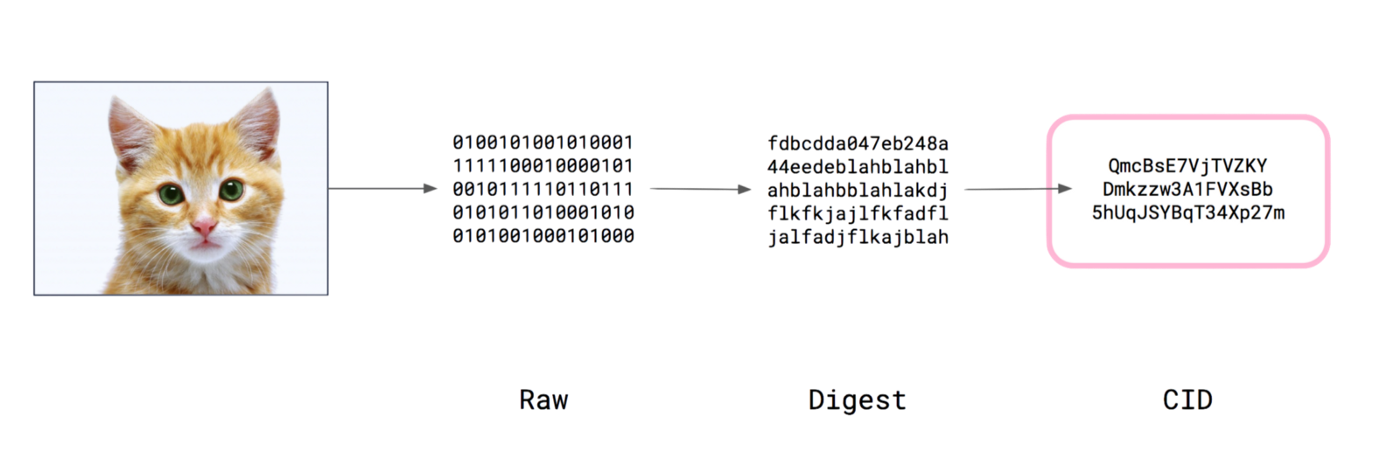
\includegraphics[width=\textwidth]{ipfs_raw_dig_cid_1.png}
    \caption{From raw image to cryptographic digest to content id (multihash).}
    \label{img:ipfsalgorithmvis1}
  \end{subfigure}
  \hfill
  \begin{subfigure}[!hbtp]{0.45\textwidth}
    \centering
    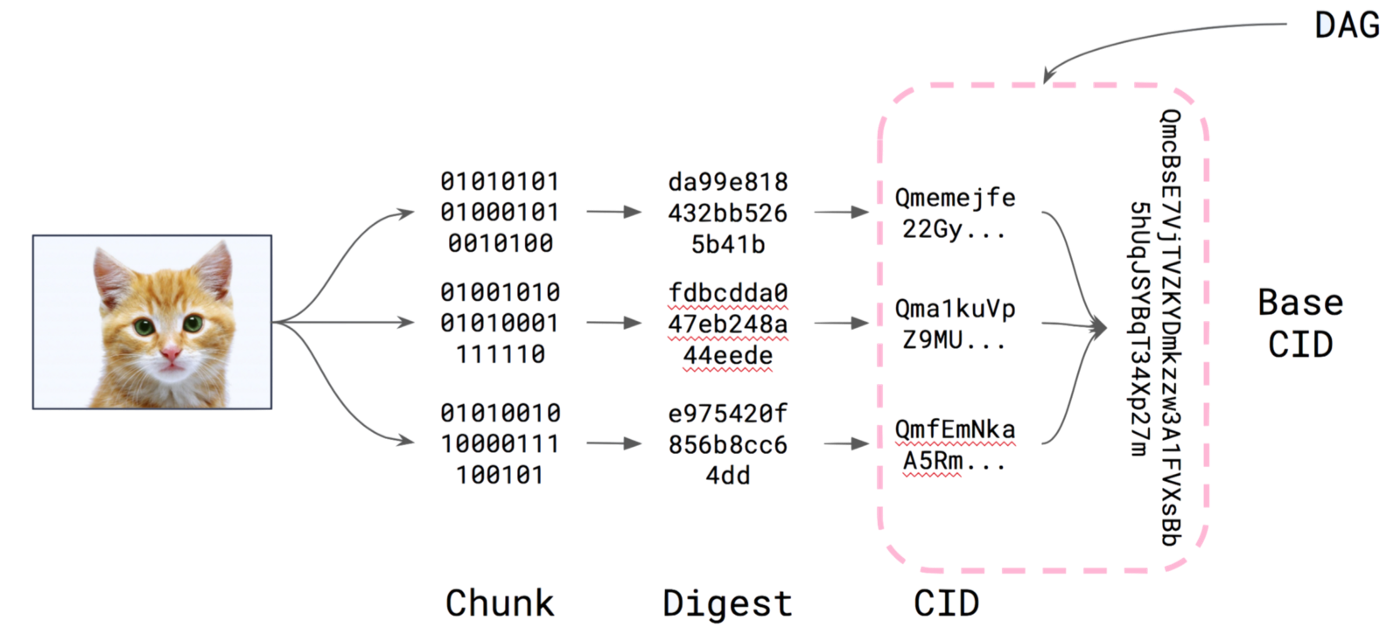
\includegraphics[width=\textwidth]{ipfs_raw_dig_cid_2.png}
    \caption{Large files are chunked, hashed, and organized into an IPLD (Merkle DAG object).}
    \label{img:ipfsalgorithmvis2}
  \end{subfigure}
  \caption{IPFS base CID construction}
  \label{img:ipfsAlgorithmVis}
\end{figure}

The content is chunked up into smaller parts (about 256k each), each part is hashed, a CID is created for each chunk, and then these chunks are combined into a hierarchical data structure, for which a single, base CID is computed.
This data structure is essentially something called a Merkle DAG, or directed acyclic graph. \\[-8pt]

\subsection{Need for IPFS protocol}

Web 3.0 is a long-term target that aims to replace the current internet infrastructure. As decentralization is the essence of Web 3.0. Many consider the distributed ledger technology (DLT), for example, blockchains, as the core building block of Web 3.0. A blockchain is an immutable and append-only ledger that stores the network state. Distributed consensus between all the network nodes is required in order to extend the blockchain and store the critical network data among the network nodes. Therefore, it could be prohibitively expensive to store any other kinds of data into the blockchain. For multiple use cases, it may be more efficient to store other non-critical data in a secure fashion close to the security level of the blockchain. \\[-8pt]

IPFS is the most suitable storage medium for this category of data. IPFS allows for distributed storage of data that is immune to altering and forgery. Data stored on the IPFS network cannot be altered without changing the data identifier. In IPFS, the identifier is a cryptographic hash of the data. This means non-critical data can be stored to IPFS while storing this identifier to an underlying distributed ledger. This would result in less exhaustive operations over the distributed ledger. \\[-8pt]

\subsection{The Optimal Storage Platform for dApps}

Decentralized applications (dApps) are a class of applications that leverage decentralization to achieve unprecedented benefits. Among those are decentralized exchanges and marketplaces where centralized intermediaries are removed, hence eliminating/reducing any trading fees. Another example is decentralized social media and video platforms where content cannot be censored at the will of the operating company. Such dApps require the storage of a significant amount of data. IPFS allows this data to be stored in a distributed way that is censorship-resistant. For these reasons, IPFS is turning into a preferred storage platform for dApps.
%%% Local Variables:
%%% mode: latex
%%% TeX-master: t
%%% End:

\section{The Necessity of Blockchain}

\subsection{What is Blockchain}

A blockchain is a growing list of records, called blocks, that are securely linked together using cryptography. Each block contains a cryptographic hash of the previous block, a timestamp, and transaction data (generally represented as a Merkle tree, where data nodes are represented by leafs). The timestamp proves that the transaction data existed when the block was published to get into its hash. As blocks each contain information about the block previous to it, they form a chain, with each additional block reinforcing the ones before it. Therefore, blockchains are resistant to modification of their data because once recorded, the data in any given block cannot be altered retroactively without altering all subsequent blocks. \\[-8pt]

Blockchains are typically managed by a peer-to-peer network for use as a publicly distributed ledger, where nodes collectively adhere to a protocol to communicate and validate new blocks. Although blockchain records are not unalterable as forks are possible, blockchains may be considered secure by design and exemplify a distributed computing system with high Byzantine fault tolerance.

\input{resources/figures/bitcoin_blockchain_structure}

\subsection{Blockchain in The Cloud Storage Use Case}

For the system to be completely decentralized, we do not use centralized databases owned by a single entity, but we use Blockchain to keep track of users' files' metadata. \\[-8pt]

The immutable nature of blockchain, and the fact that every computer on the network is continually verifying the information stored on it, makes blockchain an excellent tool for storing data. \\[-8pt]

The blockchain will help reduce the security and data loss concerns associated with a typical public storage solution. Also, it will help reduce downtime on the cloud. Users with excess storage will have the option of renting out their spaces for a fee. \\[-8pt]

\noindent
There are many advantages to using blockchain technology compared to other traditional technologies listed below. \\

\begin{itemize}
\item \textbf{Transparency: } Blockchain makes transaction histories more transparent than they ever were. Because it is a type of a distributed ledger, all nodes in the network share a copy of the documentation.  The data on a blockchain ledger is easily accessible for everyone to view. If a transaction history changes, everyone in the network can see the change and the updated record. Therefore, all information about currency exchange is available to everyone. \\
\item \textbf{Security: } Blockchain is better than any other record-keeping system when it comes to security, by all standards. The shared documentation of transactions can only be updated and/or modified with consensus on a blockchain network. Only if everyone or a majority of nodes agree to update a record, the information is edited. Moreover, when a transaction is approved, it is encrypted and connected with the previous transaction. Therefore, no one person or party has the potential to alter a record.\\
\item \textbf{Traceability: } In complex supply chains, it is hard to trace products back to their origins. But, with blockchain, the exchanges of goods are recorded, so you get an audit trail to learn where a particular asset came from.\\
\item \textbf{Cost reduction: } As blockchain eliminates the need for third-parties and middlemen, it saves enormous costs for businesses. Given that you can trust the trading partner, you don’t need anyone else to establish the rules and policies of exchange.\\
\end{itemize}
%%% Local Variables:
%%% mode: latex
%%% TeX-master: t
%%% End:

\section{Infura, The Blockchain Node as a Service}

When the transaction is signed, it has to be broadcasted to the blockchain network so miners know it and can include it in the block. \\[-8pt]

By connecting the wallet to a blockchain node, the node can run locally or connect to an Infura node. Infura takes care of keeping the nodes upgraded, online, and scaled; it handles as many transactions as you send to it. This is what Metamask does. Metamask sends all signed transactions through Infura nodes to the Ethereum network. \\[-8pt]

All blockchain nodes constantly communicate in-real time using peer-to-peer protocols. Peers exchange information about other peers, blocks, and transactions. When Infura nodes receive your signed transaction, Infura nodes propagate it further to other nodes and miners. \\[-8pt]

\input{resources/figures/infura_propagate}

%%% Local Variables:
%%% mode: latex
%%% TeX-master: t
%%% End:

\section{Metamask, The Wallet Auth}

To transact on Ethereum, you need an account. There is no MySQL ``users'' table. There is no email/password login. \\[-8pt]

To create an Ethereum account, you need to set up a crypto wallet like Metamask. The wallet will be responsible for generating and securing your crypto keys for signing transactions. \\[-8pt]

Metamask generates your Private Key. You derive the Public Key from the Private Key. Your account's address is the last 20 bytes of a hashed Public Key. \\[-8pt]

\input{resources/figures/ecdsa_generate_key}

The JS libraries will then connect to your Metamask wallet (if you permit them to do so), and they will ask you to sign Ethereum transactions. A decentralized application can't do anything without your signature.

Figure \ref{img:transactionFlowDig} show the transaction flow diagram.

\input{resources/figures/transaction_flow_diagram}
%%% Local Variables:
%%% mode: latex
%%% TeX-master: t
%%% End:

\section{Methodology}

\input{parts/main/background_materials/methodology/usecase_modeling}

	\chapter{System Design}

\section{Introduction}

The current standard for digital data storage is called cloud storage. With cloud storage, users looking to host data, applications, and websites on the internet are reliant on centralized providers like Amazon, Google, and Microsoft to provide storage services. This method of storage — for which user data is stored on the centralized server farms of cloud storage providers — is often cheaper, more scalable, and more readily accessible across geographic regions than the previous standard of storage on physical hardware.

Cloud service providers allow developers to launch their applications more quickly, without worrying about setting up and managing servers, but customers typically have limited options in terms of providers and functionality. The majority of cloud storage providers are subsidiaries of bonafide tech giants and dominate the cloud services market, accounting for about 70\% of the total market share as of 2021.

Despite their popularity and widespread use, many centralized cloud storage providers have been criticized for their tendency to force end users into inflexible and expensive cloud services and storage plans due to a lack of viable alternatives. Studies have shown that many developers settle for fixed amounts of hosting space that remain underutilized. This often results in hefty — and in many cases, unnecessary — premiums paid for cloud services.

That said, perhaps the biggest concern with centralized data storage models is that users are required to place trust in the central authority of the provider to keep their data safe, keep websites online, and not tamper with or censor the content that the centralized data providers host. In response, blockchain technology and decentralized networks have fostered a whole new methodology for digital storage: decentralized cloud storage.

In contrast to centralized, permissioned cloud providers, decentralized cloud storage providers leverage infrastructure that is designed to mitigate undue control or influence. These providers typically also utilize a permissionless structure that enables developers to employ their services with reduced restrictions. Conceptually similar to a decentralized blockchain, decentralized storage models draw their security from their widely distributed structure. This overall architecture can help make these systems more resistant to the hackers, attacks, and outages that have plagued large, centralized data centers.
%%% Local Variables:
%%% mode: latex
%%% TeX-master: t
%%% End:

\section{System Architecture}

Here is the conceptual model that defines the structure, behavior, and more views of a system.

\input{resources/figures/system_architecture}

%%% Local Variables:
%%% mode: latex
%%% TeX-master: t
%%% End:

\subsection{Tools and Technologies}

\begin{longtable}{p{0.15\linewidth} | p{0.80\linewidth}}
  \caption{Tools and technologies used in this project}
  \label{tab:toolsAndTech}
  \\\toprule
  \centering
  Tool & justification
  \\\midrule
  JavaScript & {
    JavaScript, often abbreviated JS, is a programming language that is one of the core technologies of the World Wide Web, alongside HTML and CSS. As of 2022, 98\% of websites use JavaScript on the client side for web page behavior, often incorporating third-party libraries. All major web browsers have a dedicated JavaScript engine to execute the code on users' devices.
  }
  \\\hline
  Next.js & {
    Next.js is an open-source web development framework built on top of Node.js enabling React-based web applications functionalities such as server-side rendering and generating static websites. React documentation mentions Next.js among ``Recommended Toolchains'' advising it to developers as a solution when ``Building a server-rendered website with Node.js''. Where traditional React apps can only render their content in the client-side browser, Next.js extends this functionality to include applications rendered on the server-side.
  }
  \\\hline
  Solidity & {
    Solidity is an object-oriented programming language for implementing smart contracts on various blockchain platforms, most notably, Ethereum. It was developed by Christian Reitwiessner, Alex Beregszaszi, and several former Ethereum core contributors. Programs in Solidity run on Ethereum Virtual Machine.
  }
  \\\hline
  Ethers.js & {
    The ethers.js library aims to be a complete and compact library for interacting with the Ethereum Blockchain and its ecosystem. It was originally designed for use with ethers.io and has since expanded into a more general-purpose library.
  }
  \\\hline
  Metamask & {
    MetaMask is a software cryptocurrency wallet used to interact with the Ethereum blockchain. It allows users to access their Ethereum wallet through a browser extension or mobile app, which can then be used to interact with decentralized applications. MetaMask is developed by ConsenSys Software Inc., a blockchain software company focusing on Ethereum-based tools and infrastructure.
  }
  \\\hline
  Hardhat & {
    Hardhat is an Ethereum development environment. Compile your contracts and run them on a development network. Get Solidity stack traces, console.log and more.
  }
  \\\hline
  IPFS & {
    The InterPlanetary File System (IPFS) is a protocol and peer-to-peer network for storing and sharing data in a distributed file system. IPFS uses content-addressing to uniquely identify each file in a global name-space connecting all computing devices.
  }
  \\\hline
  Docker & {
    Docker is a set of platform as a service (PaaS) products that use OS-level virtualization to deliver software in packages called containers. We use docker for shipping and self-hosting the dApp.
  }
  \\\hline
  Ropsten & {
    Ropsten Ethereum (also known as ``Ethereum Testnet'') is an Ethereum test network that allows for blockchain development testing before deployment on Mainnet, the main Ethereum network. Testnet ethers are separate and distinct from actual ethers, and are never supposed to have any value. This allows application developers or Ethereum testers to experiment, without having to use real ethers or worrying about breaking the main Ethereum chain.
  }
  \\\bottomrule
\end{longtable}

\section{Implementation and Testing}

Here you will find the implementation details.

\subsection{Smart Contracts}

\subsubsection{States}

Persistent data is referred to as storage and is represented by state variables. These values get stored permanently on the blockchain. You need to declare the type so that the contract can keep track of how much storage on the blockchain it needs when it compiles.

\lstinputlisting[style=solidity]{resources/codes/sm_states.sol}

\subsubsection{Store File}

Whenever you call storeFile with its parameters, it pushes a new file to the array of files of the account that makes that call.
\lstinputlisting[style=solidity]{resources/codes/sm_storeFile.sol}

\subsubsection{Retrieve File}

getFiles are a group of functions that retrieve the files' metadata.
\lstinputlisting[style=solidity]{resources/codes/sm_getFiles.sol}

\subsubsection{Share File}

Whenever you call shareFile with the address parameter, it pushes a new file to the array of files of that address.
\lstinputlisting[style=solidity]{resources/codes/sm_shareFile.sol}

\subsubsection{Delete File}

Whenever you call deleteFile with the index parameter, it removes the file with that index from the array of files of the account that makes that call.
\lstinputlisting[style=solidity]{resources/codes/sm_deleteFile.sol}

\subsection{Front End}


\subsubsection{Initialize}

The initialize function is executed whenever the user clicks the connect wallet button.
\lstinputlisting[style=javascript]{resources/codes/fe_initialize.js}

\subsubsection{UploadFile}

When you press the upload button, this is what happens: \\
\begin{itemize}
\item The file gets encrypted using AES-256-CBC mode.
\item The file is split into small chunks and uploaded to the IPFS node.
\item The file's metadata is stored in the smart contract.
\end{itemize}

\lstinputlisting[style=javascript]{resources/codes/fe_uploadFile.js}


	\chapter{Results and Discussion}

\section{Results}

% Results: you should assess the success of your project. How does it compare with the
% original specification? How reliable is it? How have you tested it? Comment on its
% robustness. This is done in the final documentation of the project.

We tested the Devault with uploading, downloading, sharing, deleting, connecting, and disconnecting functionality on different browsers and devices. Below we show the results of three of these tests. \\

\noindent
\textbf{1. \textit{Brave browser, the desktop version and metamask}} \\

Figure \ref{img:connectResult} shows the result of connecting the wallet.

\input{resources/figures/connect_result}

\newpage
\noindent
\textbf{2. \textit{Brave browser, the mobile version and brave wallet}} \\

Figure \ref{img:uploadResult} shows the result of uploading files functionality.

\input{resources/figures/upload_result}

\newpage
\noindent
\textbf{3. \textit{Firefox browser, the desktop version and metamask}} \\

Figure \ref{img:shareResult} shows the result of sharing files functionality.

\input{resources/figures/share_result}

\newpage
\subsection{Performance}

For performance testing we used GTmetrix tool.

GTmetrix is one of the most popular tools for analyzing site speed performance. If you put a website to the test, it will provide a performance score and a report which shows the current state of the site along with some suggestions on what can be improved.
Figure \ref{img:gtmetrixTest} shows performance of devault has reached the highest grade.

\input{resources/figures/gtmetrix}

\begin{table}[!ht]
  \centering
  \caption{The performance report details}
  \begin{tabular}{p{0.35\linewidth} p{0.35\linewidth}}
    \toprule
    Performance Metrics & The measure
    \\\midrule
    Total Page Size & 450KB. \\
    Total Page Requests & 31. \\
    Fully Loaded Time & 370ms. \\
    Largest Content Element & 306ms
    \\\bottomrule
  \end{tabular}
\end{table}
\section{Discussion}

% Discussion: here you will summarize your achievements and also the deficiencies of
% your project. You can also say what you would or could have done, if you had had more
% time or if things had worked out differently. It is important to be completely honest
% about the deficiencies and inadequacies of your work, such as they are. Part of your aim
% is to demonstrate your ability to recognize problems that remain. This is done in GP2.

	\chapter{Conclusion and Future Work}

\section{Conclusion}

Blockchain is quite a buzz word right now, but once we really understand it and how it can make many applications we know and work with regularly more effective and efficient, we’ll realize its true power.

All in all, a decentralized cloud storage app is more secure, faster, more efficient for file storage through apps like IPFS, and less costly to use than traditional decentralized file storage.

\section{Future Work}

\begin{enumerate}
\item Support Arabic language.
\item Use Shamir's Secret Sharing algorithms for sharing files.
\item Add the search functionality.
\item Compress files before uploading.
\item Enhance the ui/ux.
\item Manipulate selected files and folders.
\item Deploy to the mainnet.
\item Use Filecoin instead of IPFS.
\item Use the advantages of private and public keys in encryption/decryption.
\item Give feedback if the key used for decryption is not the same key used for encryption.
\end{enumerate}
  \section{Future Work}

\begin{enumerate}
\item Support Arabic language.
\item Use Shamir's Secret Sharing algorithms for sharing files.
\item Add the search functionality.
\item Compress files before uploading.
\item Enhance the ui/ux.
\item Manipulate selected files and folders.
\item Deploy to the mainnet.
\item Use Filecoin instead of IPFS.
\item Use the advantages of private and public keys in encryption/decryption.
\item Give feedback if the key used for decryption is not the same key used for encryption.
\end{enumerate}

	\part*{Appendix}
\addcontentsline{toc}{part}{Appendix}
  \chapter*{Glossary}
\addcontentsline{toc}{chapter}{Glossary}

\printglossary[
type=\acronymtype,
style=long,
title=Acronyms,
toctitle=Acronyms
]

\printglossary[
type=main,
style=long,
title=Terminology,
toctitle=Terminology
]

\glsaddall
  \addcontentsline{toc}{chapter}{Lists}

  \listoffigures
\addcontentsline{toc}{section}{\listfigurename}
  \listoftables
\addcontentsline{toc}{section}{\listtablename}
  % \printbibheading
% \printbibliography[type=book, heading=bibintoc, title={Books}]

\addcontentsline{toc}{chapter}{References}

\nocite{*}

\printbibliography
\end{document}

	\section{Introduction}

The current standard for digital data storage is called cloud storage. With cloud storage, users looking to host data, applications, and websites on the internet are reliant on centralized providers like Amazon, Google, and Microsoft to provide storage services. This method of storage — for which user data is stored on the centralized server farms of cloud storage providers — is often cheaper, more scalable, and more readily accessible across geographic regions than the previous standard of storage on physical hardware.

Cloud service providers allow developers to launch their applications more quickly, without worrying about setting up and managing servers, but customers typically have limited options in terms of providers and functionality. The majority of cloud storage providers are subsidiaries of bonafide tech giants and dominate the cloud services market, accounting for about 70\% of the total market share as of 2021.

Despite their popularity and widespread use, many centralized cloud storage providers have been criticized for their tendency to force end users into inflexible and expensive cloud services and storage plans due to a lack of viable alternatives. Studies have shown that many developers settle for fixed amounts of hosting space that remain underutilized. This often results in hefty — and in many cases, unnecessary — premiums paid for cloud services.

That said, perhaps the biggest concern with centralized data storage models is that users are required to place trust in the central authority of the provider to keep their data safe, keep websites online, and not tamper with or censor the content that the centralized data providers host. In response, blockchain technology and decentralized networks have fostered a whole new methodology for digital storage: decentralized cloud storage.

In contrast to centralized, permissioned cloud providers, decentralized cloud storage providers leverage infrastructure that is designed to mitigate undue control or influence. These providers typically also utilize a permissionless structure that enables developers to employ their services with reduced restrictions. Conceptually similar to a decentralized blockchain, decentralized storage models draw their security from their widely distributed structure. This overall architecture can help make these systems more resistant to the hackers, attacks, and outages that have plagued large, centralized data centers.
	\chapter{Literature Review}

\section{Proof}
See below for irrefutable proof, extreme care and rigour has been shown in this proof by \gls{evm}.\par

\namedfigure
{h}
{very_real_figure}
{
\includegraphics[width=\textwidth]{resources/images/very_important_image.jpg}}
{Clear proof of theorem.}


As stated in the \gls{dapp} theorem, I'm right.

	%%% Local Variables:
%%% mode: latex
%%% TeX-master: t
%%% End:

\section{Methodology}

%%% Local Variables:
%%% mode: latex
%%% TeX-master: t
%%% End:

\subsection{Use Case Modeling}

A use case diagram is a graphical depiction of a user's possible interactions with a system. A use case diagram shows various use cases and different types of users the system has and will often be accompanied by other types of diagrams as well.
In Devault the user can upload, download, share, delete, sort, and search files. Also the user can connect and disconnect their blockchain wallet.

\subsubsection{Use Case Diagram}

%%% Local Variables:
%%% mode: latex
%%% TeX-master: t
%%% End:
\namedfigure
{!htbp}
{img:useCaseDiagram}
{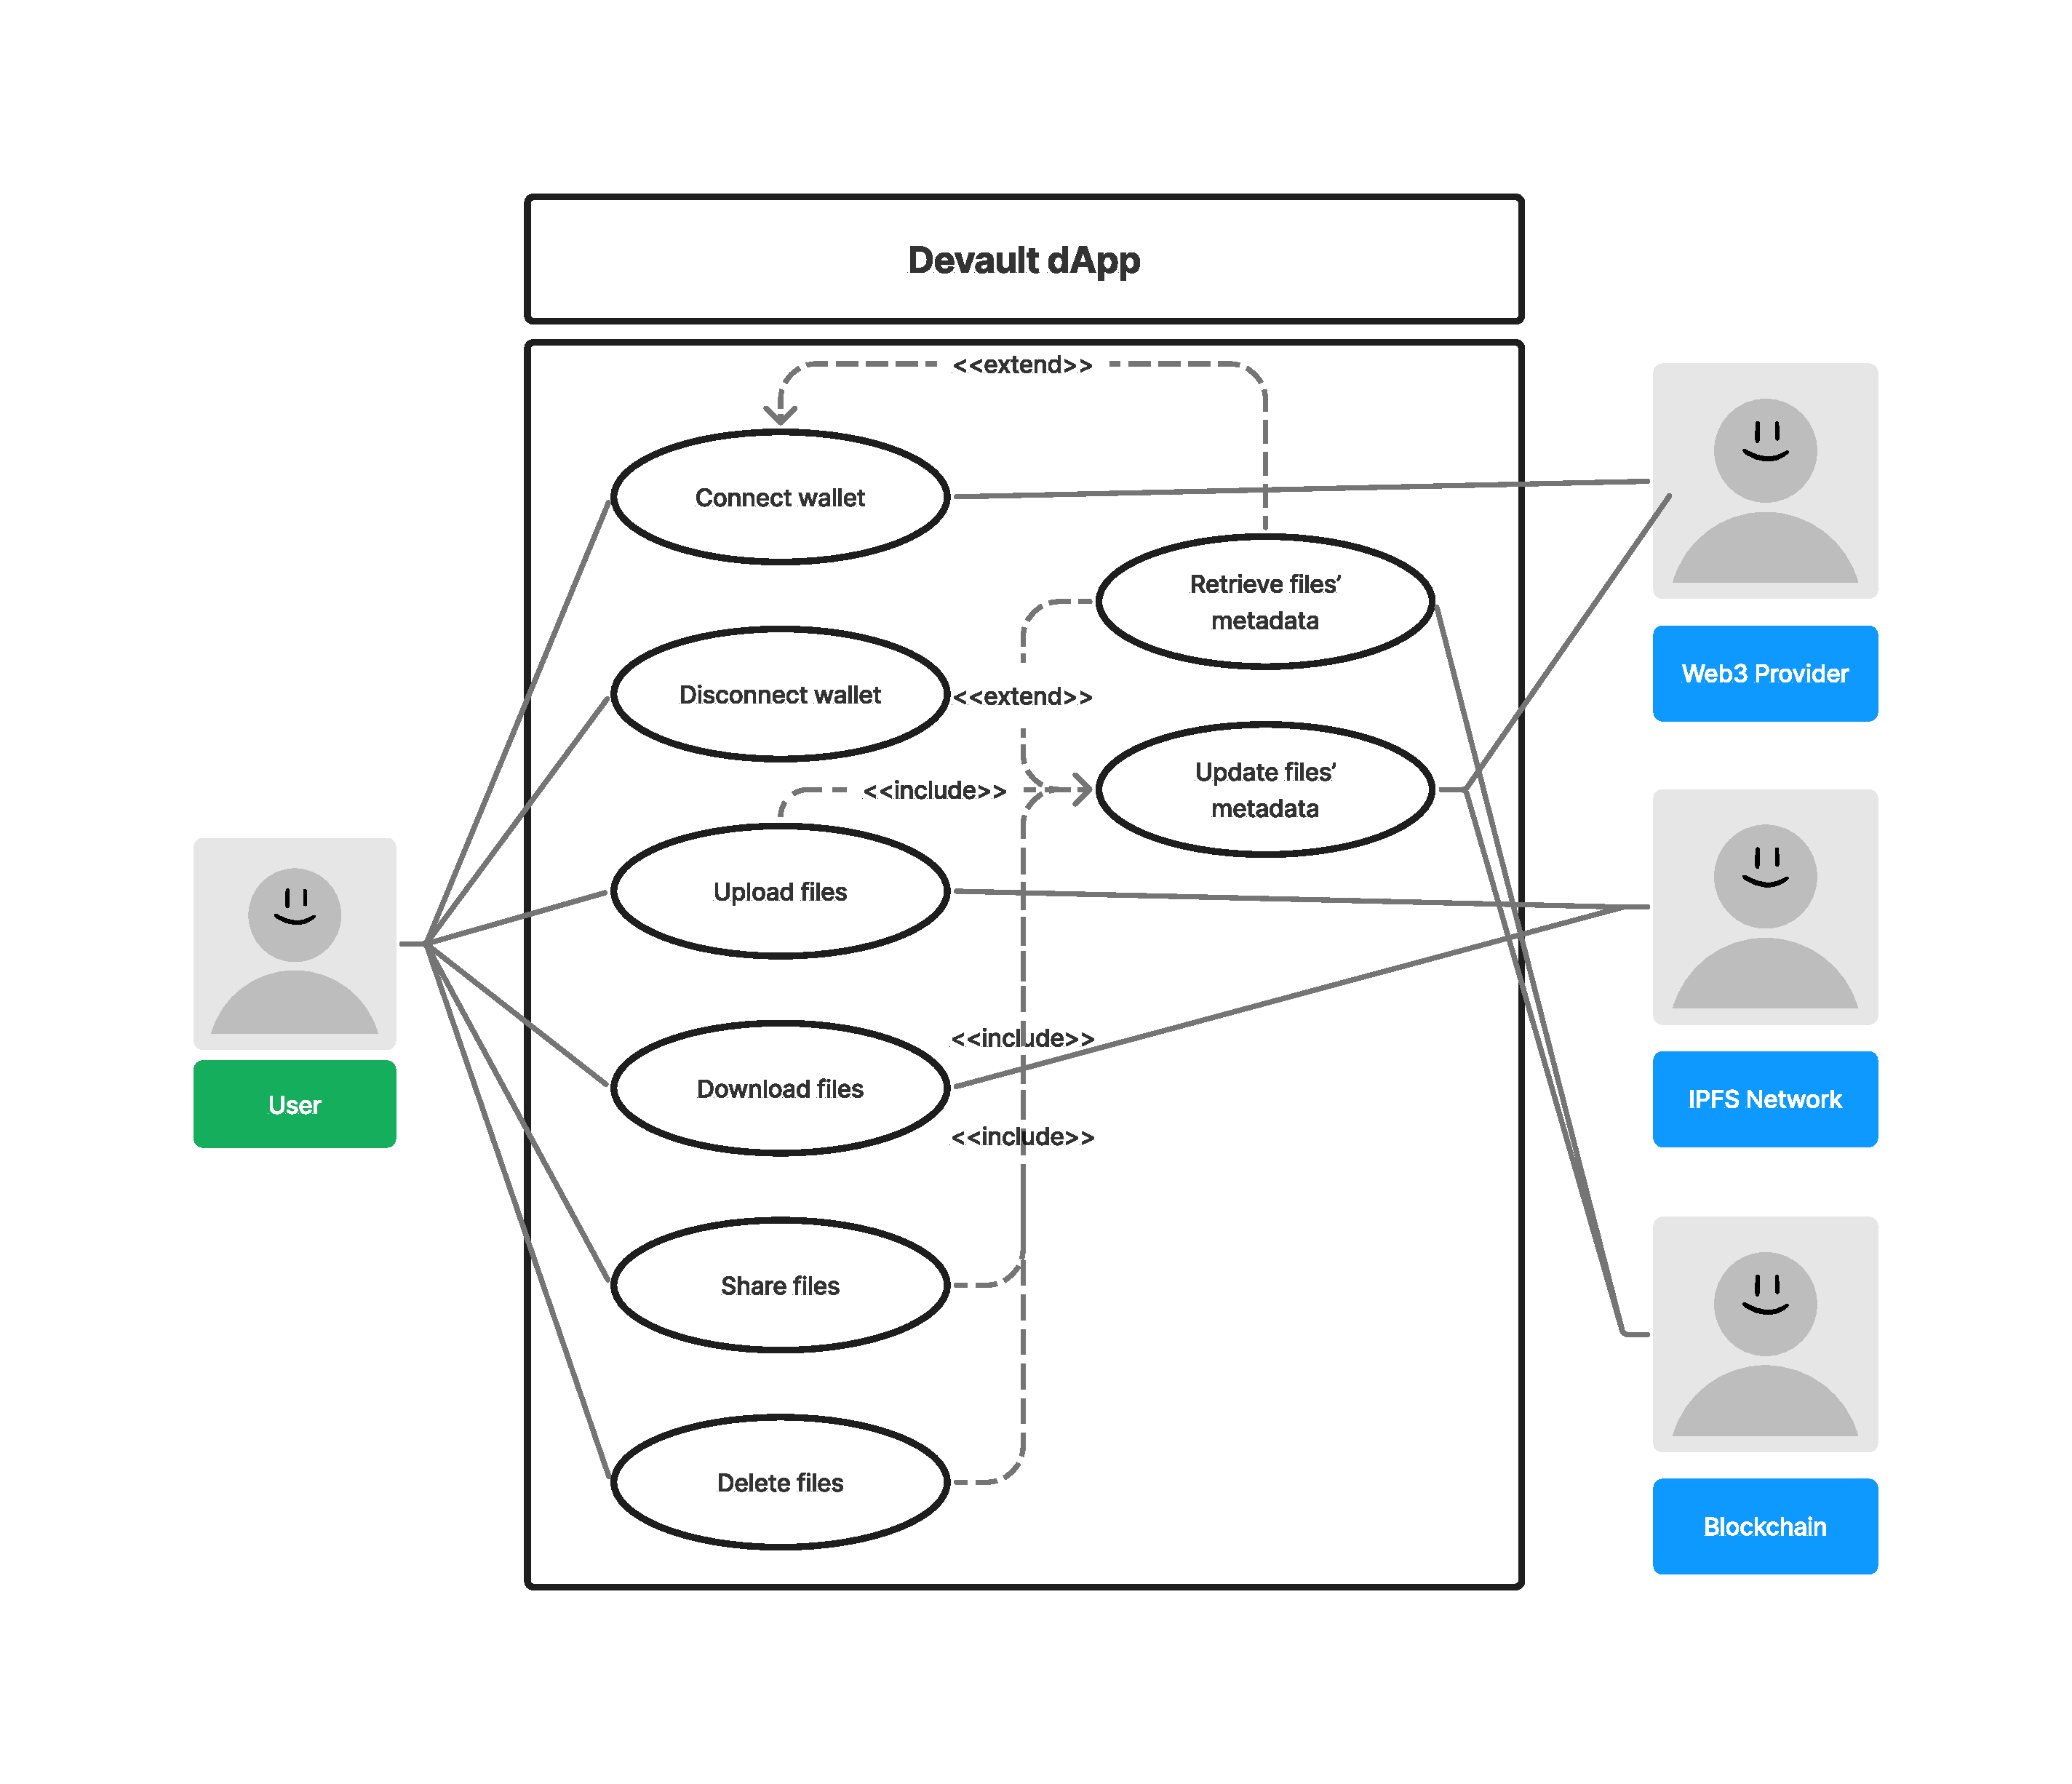
\includegraphics[width=\textwidth]{resources/images/usecases-diagram.pdf}}
{dApp use case diagram.}


\newpage

\subsubsection{Use Case Model}

\begin{longtable}{p{0.20\linewidth} | p{0.75\linewidth}}
  \caption{Use case 1: Connecting wallet}
  \label{tab:useCaseConnect}
  \\\toprule
  ID & UC\_1
  \\\midrule
  Title & \textbf{Connecting wallet}
  \\\hline
  Description & The user can connect with their Ethereum wallet to use the system.
  \\\hline
  Primary Actor & User.
  \\\hline
  Pre-Conditions & {
    \begin{itemize}
    \item The user must have internet connection.
    \item The user navigates to \url{devault.vercel.app} or any other instance.
    \end{itemize}
  }\vspace*{-\baselineskip}
  \\\hline
  Main Success Scenario & {
    \begin{enumerate}
    \item The user clicks the connect wallet button.
    \item The user confirms the connection.
    \item The system then will retrieve the files from that account.
    \end{enumerate}
  }\vspace*{-\baselineskip}
  \\\bottomrule
\end{longtable}

\begin{longtable}{p{0.20\linewidth} | p{0.75\linewidth}}
  \caption{Use case 2: Uploading files}
  \label{tab:useCaseUpload}
  \\\toprule
  ID & UC\_2
  \\\midrule
  Title & \textbf{Uploading files}
  \\\hline
  Description & The user can upload files or folders to the system.
  \\\hline
  Primary Actor & User.
  \\\hline
  Pre-Conditions & {
    \begin{itemize}
    \item UC\_1
    \end{itemize}
  }\vspace*{-\baselineskip}
  \\\hline
  Main Success Scenario & {
    \begin{enumerate}
    \item The user navigates to the vault tab.
    \item The user clicks on the upload button and picks a file or folder to upload.
    \item The user enters a password to encrypt the files.
    \item The system then will encrypt the files, store their metadata in the blockchain, and upload the encrypted files to the \gls{p2p g} network.
    \end{enumerate}
  }\vspace*{-\baselineskip}
  \\\bottomrule
\end{longtable}

\begin{longtable}{p{0.20\linewidth} | p{0.75\linewidth}}
  \caption{Use case 3: Downloading files}
  \label{tab:useCaseDownload}
  \\\toprule
  ID & UC\_3
  \\\midrule
  Title & \textbf{Downloading files}
  \\\hline
  Description & The user can download files or folders from the system.
  \\\hline
  Primary Actor & User.
  \\\hline
  Pre-Conditions & {
    \begin{itemize}
    \item UC\_1
    \end{itemize}
  }\vspace*{-\baselineskip}
  \\\hline
  Main Success Scenario & {
    \begin{enumerate}
    \item The user navigates to the vault tab.
    \item The user selects the files they need to download.
    \item The user enter a password to decrypt the files.
    \item The system then will decrypt the files and download them.
    \end{enumerate}
  }\vspace*{-\baselineskip}
  \\\bottomrule
\end{longtable}

\begin{longtable}{p{0.20\linewidth} | p{0.75\linewidth}}
  \caption{Use case 4: Sharing files}
  \label{tab:useCaseShare}
  \\\toprule
  ID & UC\_4
  \\\midrule
  Title & \textbf{Sharing files}
  \\\hline
  Description & The user can share files or folders with other users.
  \\\hline
  Primary Actor & User.
  \\\hline
  Pre-Conditions & {
    \begin{itemize}
    \item UC\_1
    \end{itemize}
  }\vspace*{-\baselineskip}
  \\\hline
  Main Success Scenario & {
    \begin{enumerate}
    \item The user navigates to the vault tab.
    \item The user selects the files they need to share.
    \item The user clicks the share button.
    \item The user will be prompted to enter the addresses to share the file.
    \item The system then will share the files with these addresses.
    \end{enumerate}
  }\vspace*{-\baselineskip}
  \\\bottomrule
\end{longtable}

\begin{longtable}{p{0.20\linewidth} | p{0.75\linewidth}}
  \caption{Use case 5: Deleting files}
  \label{tab:useCaseDelete}
  \\\toprule
  ID & UC\_5
  \\\midrule
  Title & \textbf{Deleting files}
  \\\hline
  Description & The user can Delete files or folders form the system.
  \\\hline
  Primary Actor & User.
  \\\hline
  Pre-Conditions & {
    \begin{itemize}
    \item UC\_1
    \end{itemize}
  }\vspace*{-\baselineskip}
  \\\hline
  Main Success Scenario & {
    \begin{enumerate}
    \item The user navigates to the vault tab.
    \item The user selects the files they need to delete.
    \item The user clicks the delete button.
    \item The user will be prompted to confirm the deletion process.
    \item The system then will delete the files with form the user address.
    \end{enumerate}
  }\vspace*{-\baselineskip}
  \\\bottomrule
\end{longtable}

\begin{longtable}{p{0.20\linewidth} | p{0.75\linewidth}}
  \caption{Use case 6: Disconnecting wallet}
  \label{tab:useCaseDisconnect}
  \\\toprule
  ID & UC\_6
  \\\midrule
  Title & \textbf{Connecting wallet}
  \\\hline
  Description & The user can disconnect their Ethereum wallet from the system.
  \\\hline
  Primary Actor & User.
  \\\hline
  Pre-Conditions & {
    \begin{itemize}
    \item UC\_1
    \end{itemize}
  }\vspace*{-\baselineskip}
  \\\hline
  Main Success Scenario & {
    \begin{enumerate}
    \item The user clicks the disconnect wallet button.
    \item The system will log this user out.
    \end{enumerate}
  }\vspace*{-\baselineskip}
  \\\bottomrule
\end{longtable}

	\chapter{System Development Methodology}
	\chapter{Result and Analysis}
  \section{Future Work}

\begin{enumerate}
\item Support Arabic language.
\item Use Shamir's Secret Sharing algorithms for sharing files.
\item Add the search functionality.
\item Compress files before uploading.
\item Enhance the ui/ux.
\item Manipulate selected files and folders.
\item Deploy to the mainnet.
\item Use Filecoin instead of IPFS.
\item Use the advantages of private and public keys in encryption/decryption.
\item Give feedback if the key used for decryption is not the same key used for encryption.
\end{enumerate}
  \chapter{Limitations}

\gls{genesis}
\gls{consensus}
\gls{blockchain}
\gls{nonce}


	\part*{Appendix}
\addcontentsline{toc}{part}{Appendix}
  \chapter*{Glossary}
\addcontentsline{toc}{chapter}{Glossary}

\printglossary[
type=\acronymtype,
style=long,
title=Acronyms,
toctitle=Acronyms
]

\printglossary[
type=main,
style=long,
title=Terminology,
toctitle=Terminology
]

\glsaddall
  \addcontentsline{toc}{chapter}{Lists}

  \listoffigures
\addcontentsline{toc}{section}{\listfigurename}
  \listoftables
\addcontentsline{toc}{section}{\listtablename}
  % \printbibheading
% \printbibliography[type=book, heading=bibintoc, title={Books}]

\addcontentsline{toc}{chapter}{References}

\nocite{*}

\printbibliography
\end{document}
